\chapter{Simulaci\'on de flujo multif\'asico}
\label{chap:isot}

\section{Lattice Boltzmann para flujo multif\'asico}
En sinton\'ia con el crecimiento de la mec\'anica de fluidos computacional, fueron desarroll\'andose numerosos m\'etodos num\'ericos macrosc\'opicos destinados a resolver las ecuaciones de Navier-Stokes en flujos multif\'asicos \cite{scardovelli_direct_1999}. Entre los m\'etodos m\'as populares, pueden destacarse el de \textbf{front-tracking}, el m\'etodo Volume of Fluid (VOF) y el m\'etodo level set. A pesar de la amplia difusi\'on adquirida, y de la demostrada capacidad para resolver con precisi\'on diversos escenarios con flujos multif\'asicos, estas t\'ecnicas tradicionales contin\'uan presentando limitaciones que dificultan el modelado de problemas complejos con transferencia de calor, como ebullici\'on y condensaci\'on. En particular, el m\'etodo de \textbf{front-tracking} generalmente no permite simular adecuadamente procesos de coalescencia y ruptura de una interfase \cite{scardovelli_direct_1999,liu_three-dimensional_2012}. La aplicaci\'on de VOF y level set suele requerir pasos de reconstrucci\'on o reinicializaci\'on de la interfase, que pueden no ser f\'isicos y complejos de implementar \cite{liu_three-dimensional_2012}. Adem\'as, suelen originarse inestabilidades num\'ericas en el uso de VOF o level set para simular flujos dominados por tensi\'on superficial en geometr\'ias complejas \cite{scardovelli_direct_1999}.
\par
En comparaci\'on con otros m\'etodos computacionales, el MLB presenta ventajas adicionales para la simulaci\'on de flujos complejos. Por un lado, la naturaleza mesosc\'opica con base en la teor\'ia cin\'etica molecular permite generar modelos con s\'olidos fundamentos termodin\'amicos. Por otro lado, es posible incorporar directamente el uso de ecuaciones de estado en la resoluci\'on de Navier-Stokes en escala macrosc\'opica, lo que a su vez elimina la necesidad de resolver una ecuaci\'on de Poisson para la presi\'on. Finalmente, la mayor\'ia de los modelos son sencillos de programar, y la naturaleza local de las operaciones involucradas facilita la explotaci\'on de arquitecturas con paralelismo masivo, como las unidades de procesamiento gr\'afico (GPU).
\par 
Las mencionadas caracter\'isticas han motivado el desarrollo de esquemas para flujo multif\'asico desde los or\'igenes del m\'etodo. A pesar de que se ha conformado un enorme universo de modelos diferentes, la gran mayor\'ia de estas alternativas pueden agruparse dentro de cuatro categor\'ias principales: color-gradient \cite{liu_three-dimensional_2012,gunstensen_lattice_1991}, pseudopotential \cite{shan_lattice_1993,shan_simulation_1994,chen_critical_2014}, free-energy \cite{swift_lattice_1996,inamuro_galilean_2000} y phase-field \cite{he_lattice_1999,liang_phase-field-based_2014}. 

\subsection*{Color-gradient}
El m\'etodo color-gradient fue introducido por Gunstensen et al. \cite{gunstensen_lattice_1991}, como una versi\'on mejorada del modelo LGA multif\'asico de Rothman y Keller \cite{rothman_immiscible_1988}. En este modelo las fases se denotan con diferentes colores, y la interacci\'on entre part\'iculas, responsable de la separaci\'on de fases, es modelada con gradientes locales de color asociado a la diferencia de densidad entre ambas fases. Tomando como ejemplo un sistema de dos fases, el modelo color-gradient original usa dos tipos de funciones de distribuci\'on, $f_{ri}$ y $f_{bi}$, para representar a los fluidos rojo y azul respectivamente. La distribuci\'on total de la mezcla $f_i = f_{ri}+f_{bi}$ evoluciona como:
\begin{equation}
	f_i(\bm{x}+\bm{e}_i\delta_t,t+\delta_t) - f_i(\bm{x},t) = \Omega_i^c + \Omega_i^p,
\end{equation}
donde $\Omega_i^c$ denota los efectos de colisi\'on y $\Omega_i^p$ se encuentra relacionado con la tensi\'on interfacial. En este caso, las densidades y velocidades para cada fase se definen como
\begin{equation}
	\begin{gathered}
	\rho_k = \sum_i f_{ki}, \qquad \rho_k\bm{u}_k = \sum_i \bm{e}_if_{ki}, \qquad k=r,b, \\
	\rho = \rho_r + \rho_b, \qquad \rho\bm{u} = \rho_r\bm{u}_r + \rho_b\bm{u}_b.
	\end{gathered}
\end{equation}

Si bien es posible emplear un operador LBGK para $\Omega_i^c$, el t\'ermino $\Omega_i^p$ se calcula empleando un par\'ametro de orden que tiene en cuenta la diferencia de densidad entre fases. Despu\'es de la colisi\'on, las funciones de distribuci\'on parciales son sometidas a un paso de ajuste de color antes del streaming. Estos pasos adicionales del algoritmo contribuyen a producir inestabilidades num\'ericas, a la vez que reducen de forma dr\'astica la eficiencia computacional por paso de tiempo \cite{guo_lattice_2013}.

\subsection*{Free-energy}
El m\'etodo free-energy fue propuesto originalmente por Swift et al. \cite{swift_lattice_1996}, y presenta un punto de partida asociado a consideraciones termodin\'amicas b\'asicas. La idea detr\'as de estos m\'etodos consiste en derivar una funci\'on de distribuci\'on de equilibrio adecuada, de forma que el momento de segundo orden correspondiente incluya un tensor de presi\'on termodin\'amico no ideal. En particular, este tensor se deriva a partir de la energ\'ia libre de un fluido asociado a una ecuaci\'on de estado de Van der Waals, y puede escribirse como:
\begin{equation}
	P^{'}_{\alpha\beta}=p\delta_{\alpha\beta}+\kappa\dfrac{\partial \rho}{\partial x_{\alpha}}\dfrac{\partial \rho}{\partial x_{\beta}}
\end{equation}
donde $\kappa$ es una constante asociada al valor de tensi\'on superficial en la interfase. Para lograr la recuperaci\'on de este tensor, Swift et al. sugirieron el uso de una ELB con operador de colisi\'on LBGK
\begin{equation}
	f_i(\bm{x}+\bm{e}_i\delta_t,t+\delta_t) - f_i(\bm{x},t) = -\dfrac{1}{\tau}\left[ f_i - f_i^{eq}(\rho, \bm{u}, \nabla\bm{u}) \right],
\end{equation}
mientras que la distribuci\'on de equilibrio satisface las siguientes restricciones:
\begin{equation}
	\sum_i f_i^{eq} = \rho, \qquad \sum_i \bm{e}_if_{i}=\rho\bm{u}, \qquad
	\sum_i \bm{e}_i\bm{e}_if_{i}= \bm{P}^{'}+\rho\bm{u}\bm{u}
	\label{eq:free_energy+rest}
\end{equation}

De forma similar a lo que ocurre con el modelo est\'andar para flujos de una \'unica fase, $f^{eq}$ puede escribirse como un polinomio de $\bm{u}$:
\begin{subequations}
	\begin{equation}
		f_i^{eq}=A + B(\bm{e}_i \cdot \bm{u}) + C u^2 + D(\bm{e}_i \cdot \bm{u})^2 + G:\bm{e}_i\bm{e}_i, \qquad i\neq 0,
	\end{equation}
	\begin{equation}
		f_i^{eq}=A_0 + C_0 u^2, \qquad i = 0.
	\end{equation}
\end{subequations}

Los coeficientes de $f_i^eq$ para una grilla bidimensional pueden obtenerse empleando las restricciones de la \eq{eq:free_energy+rest}:
\begin{equation}
	\begin{gathered}
		A_0 = \rho - 6 A, \qquad C_0 = -\rho, \\
		A = \dfrac{1}{3}(p_0-\kappa \rho \nabla^2 \rho), \qquad B = \dfrac{\rho}{3}, \qquad C = -\dfrac{\rho}{6}, \qquad  D = \dfrac{2\rho}{3},  \\
		G_{xx} = -G_{yy} = \dfrac{\kappa}{3}\left[ \left(\dfrac{\partial \rho}{\partial x}\right)^2 - \left(\dfrac{\partial \rho}{\partial y}\right)^2 \right], \qquad G_{xy}=\dfrac{2\kappa}{3}\dfrac{\partial \rho}{\partial x} \dfrac{\partial \rho}{\partial y}.
	\end{gathered}
\end{equation}

De esta forma, las ecuaciones macrosc\'opicas recuperadas usando el m\'etodo de Swift resultan:
\begin{equation}
	\dfrac{\partial \rho}{\partial t} + \nabla \cdot (\rho \bm{u}) = 0,
\end{equation}
\begin{align}
	\dfrac{\partial \rho \bm{u}}{\partial t} + \nabla \cdot (\rho \bm{uu}) =& -\nabla p_0 + \nu \nabla^2 (\rho \bm{u})+\nabla[\lambda \nabla \cdot (\rho \bm{u})]		\\
	&-\left( \tau - \dfrac{1}{2} \right)\dfrac{\partial p_0}{\partial \rho} \delta_t \nabla \cdot [\bm{u}\nabla \rho + (\nabla \rho)\bm{u}],
\end{align}
donde 
\begin{equation}
	\nu = \dfrac{\delta_t}{4}\left( \tau - \dfrac{1}{2} \right), \qquad \lambda = \delta_t\left( \tau - \dfrac{1}{2} \right)\left( \dfrac{1}{2} - \dfrac{\partial p_0}{\partial \rho}\right)
\end{equation}

\textcolor{red}{Falta decir q\'ue es $p_0$.}

Las primeras versiones asociadas a esta familia sufrieron la falta de invariancia galileana debido a la recuperaci\'on de t\'erminos que no est\'an relacionados con Navier-Stokes, originados por la misma incorporaci\'on del tensor de presi\'on en la distribuci\'on de equilibrio \cite{kuzmin_multi-relaxation_2008}. Para recuperar esta invarianza es necesario, por lo tanto, incorporar t\'erminos de correcci\'on en la funci\'on de distribuci\'on de equilibrio. Este tipo de adaptaciones son similares a aquellas adoptadas por las versiones posteriores de los m\'etodos dentro de la familia color-gradient, y usualmente constituyen fuentes adicionales de inestabilidad num\'erica al incorporar t\'erminos como $\bm{u}\nabla\rho$ y $\bm{u}\cdot\nabla\rho$.

\subsection*{Phase-field}
Esta categor\'ia representa a los modelos basados en la teor\'ia de phase-field, es decir, aquellos en los que la din\'amica de la interfase se encuentra descripta por un par\'ametro de orden regido por una ecuaci\'on de Cahn-Hilliard o similar \cite{jacqmin_calculation_1999}. Esta aproximaci\'on a la simulaci\'on de flujos multif\'asicos con LB tiene su contraparte equivalente dentro de las t\'ecnicas tradicionales de CFD para modelos de interfase difusa, como el de Ding et. al \cite{ding_diffuse_2007}.

La versi\'on original de He at al. \cite{he_lattice_1999} hace uso de dos funciones de distribuci\'on, $g$ y $f$, para recuperar las ecuaciones de Navier-Stokes y una del tipo Cahn-Hilliard para la evoluci\'on de la interfase respectivamente. Usando operadores de colisi\'on LBGK, las ecuaciones corresponden a:
\begin{equation}
	g_i(\bm{x}+\bm{e}_i\delta_t,t+\delta_t) - g_i(\bm{x},t) = -\dfrac{1}{\tau_1}\left[ g_i(\bm{x},t) - g_i^{eq}(\bm{x},t) \right] + S_i(\bm{x},t)\delta_t,
	\label{eq:he_g_eq}
\end{equation}
\begin{equation}
	f_i(\bm{x}+\bm{e}_i\delta_t,t+\delta_t) - f_i(\bm{x},t) = -\dfrac{1}{\tau_2}\left[ f_i(\bm{x},t) - f_i^{eq}(\bm{x},t) \right] + S_i^{'}(\bm{x},t)\delta_t,
\end{equation}
donde la viscosidad cinem\'atica se recupera mediante $\nu=(c_s^2)(\tau_1-0.5)\delta_t$, $\tau_2$ se relaciona con la mobilidad de la ecuaci\'on de Cahn-Hilliard, y $S_i$, $S_i^{'}$ son t\'erminos de fuente. Las funciones de distribuci\'on de equilibrio se definen mediante:
\begin{equation}
	g_i^{eq} = w_i\left[ p + \rho c_s^2 \left( \dfrac{e_{i\alpha}u_{\alpha}}{c_s^2}  + \dfrac{e_{i\alpha}u_{\alpha}e_{i\beta}u_{\beta}}{2c_s^4} - \dfrac{u_{\alpha}u_{\alpha}}{2c_s^2} \right)  \right]
\end{equation}
\begin{equation}
	f_i^{eq} = w_i \phi \left[ 1 +  \dfrac{e_{i\alpha}u_{\alpha}}{c_s^2}  + \dfrac{e_{i\alpha}u_{\alpha}e_{i\beta}u_{\beta}}{2c_s^4} - \dfrac{u_{\alpha}u_{\alpha}}{2c_s^2}  \right]
\end{equation}
donde $p$ corresponde a la presi\'on hidrodin\'amica. $\phi$ es el par\'ametro de orden que se utiliza, por ejemplo, para determinar la distribuci\'on de densidad:
\begin{equation}
	\rho(\phi) = \rho_g + \dfrac{\phi - \phi_g}{\phi_l - \phi_g}(\rho_l - \rho_g)
\end{equation}

En este caso, los sub\'indices $l$ y $g$ corresponden a las fases l\'iquida y gaseosa respectivamente. Las variables macrosc\'opicas del modelo de He et al. se calculan como:
\begin{equation}
	\begin{gathered}
		\phi = \sum_i f_i \\
		p = \sum_i g_i - \dfrac{\delta_t}{2} u_{\beta} \dfrac{\partial(p - \rho c_s^2)}{\partial x_{\beta}} \\
		\rho u_{\alpha}c_s^2 = \sum_i e_{i\alpha}g_i + \dfrac{\delta_t}{2}c_s^2 F_{\alpha}
	\end{gathered}
	\label{eq:he_macro_variables}
\end{equation}
donde $F_{\alpha}$ representa las fuerzas externas, incluyendo las asociadas a la tensi\'on interfacial. La expansi\'on de Chapman-Enskog de las Ecs.~\eqref{eq:he_g_eq}-\eqref{eq:he_macro_variables} muestra que las ecuaciones macrosc\'opicas recuperadas resultan:
\begin{equation}
	\begin{gathered}
		\dfrac{\partial (\rho \bm{u})}{\partial t} + \nabla \cdot (\rho \bm{uu})  = -\nabla p  + \nu \nabla \cdot \left[ \rho (\nabla\bm{u} + \nabla \bm{u}^T) \right] + \bm{F} \\
		\dfrac{\partial \phi}{\partial t} + \nabla \cdot (\phi \bm{}u) = \dfrac{1}{2} \left( 1 - \dfrac{1}{2\tau_2} \right) \nabla^2 (p - c_s^2 \phi)
	\end{gathered}
\end{equation}




\subsection*{Pseudopotential}
El m\'etodo pseudopotencial, que podr\'ia considerarse como la t\'ecnica m\'as sencilla para simular flujos multif\'asicos, fue propuesta por Shan y Chen \cite{shan_lattice_1993,shan_simulation_1994}. En este m\'etodo, las interacciones entre part\'iculas fluidas son imitadas mediante un potencial interpart\'icula, de modo que la separaci\'on de fases ocurre autom\'aticamente, sin mecesidad de recurrir a t\'ecnicas para capturar o reconstruir interfases. Este potencial es el responsable de inducir un tensor de presi\'on no ideal, diferente al del m\'etodo free-energy. La simplicidad conceptual y la elevada eficiencia computacional convirtieron a este m\'etodo en uno de los m\'as pupulares, habiendo sido utilizado con \'exito en la resoluci\'on de diversos problemas.
\par 
La ELB propuesta por Shan y Chen conserva la estructura est\'andar de los modelos de \'unica fase con operador LBGK:
\begin{equation}
	f_i(\bm{x}+\bm{e}_i\delta_t,t+\delta_t) - f_i(\bm{x},t)= -\dfrac{1}{\tau}\left[ f_i(\bm{x},t) - f_i^{eq}(\rho,\bm{u}^{eq}) \right],
\end{equation}
donde $\bm{u}^{eq}$ se conoce como velocidad de equilibrio. En este modelo, los principales momentos quedan definidos por:
\begin{equation}
	\sum_i f_i = \rho, \qquad	\sum_i \bm{e}_if_i = \rho \bm{u}^* .
\end{equation}

En este caso, la velocidad $\bm{u}^*$ es utilizada para calcular $\bm{u}^{eq}$ y la velocidad real del fluido
\begin{equation}
	\bm{u}^{eq} = \bm{u}^* + \dfrac{\bm{F}\tau}{\rho}, \qquad \bm{u} = \bm{u}^* + \dfrac{\bm{F}\delta_t}{2\rho}
\end{equation}

El modelo original de Shan y Chen introduce el uso de una fuerza de interacci\'on entre part\'iculas vecinas definida como:
\begin{equation}
	\bm{F}_{int}(\bm{x},t) = -G\psi(\bm{x},t)\sum_i w_i \psi(\bm{x}+\bm{e}_i,t)\bm{e}_i
\end{equation}
donde $G$ es un par\'ametro que controla la intensidad de la fuerza de interacci\'on y $\psi$ es un potencial dado por:
\begin{equation}
	\psi(\rho) = \rho_0 \left[ 1-\mbox{e}^{-\frac{\rho}{\rho_0}} \right],
\end{equation}
donde $\rho_0$ es una constante arbitraria.

A pesar de la evoluci\'on y mejora de los diversos modelos multif\'asicos desde sus or\'igenes, siguen existiendo diferencias significativas en las capacidades de simulaci\'on de problemas multif\'asicos din\'amicos, sobre todo cuando las relaciones de densidad entre fases ($\rho_l/\rho_g$) son elevadas. Como se menciona en el trabajo de Li et al. \cite{li_lattice_2016}, estas limitaciones pueden deberse a diferentes causas. Por un lado, existen diferencias en las cantidades f\'isicas que deben ser evualuadas a trav\'es de la interfase l\'iquido-vapor; por ejemplo densidad en el modelo free-energy y potencial en pseudopotential. Por otro lado, c\'omo se mencion\'o previamente, las familias color-gradient y free-energy necesitan correcciones adicionales para recuperar adecuadamente el comportamiento de Navier-Stokes, y como estos t\'erminos dependen expl\'icitamente del gradiente de densidad, suelen convertirse en fuentes de inestablidad num\'erica \cite{leclaire_unsteady_2014,leclaire_enhanced_2013,huang_simulations_2013}. Este hecho origina que los modelos color-gradient y free-energy encuentren severas limitaciones al momento de simular flujos con elevada relaci\'on de densidades y alto n\'umero de Reynolds, a pesar de los \'exitos observados en casos est\'aticos o cuasi-est\'aticos.

A diferencia de color-gradient y free-energy, los modelos multif\'asicos agrupados dentro de las familias phase-field y pseudopotential han sido aplicados exitosamente en la simulaci\'on de problemas con elevada relaci\'on de densidades y n\'umero de Reynolds modederados, como impacto y colisi\'on de droplets \cite{li_lattice_2013,lee_stable_2005} e incluso aplicaciones sencillas de transferencia de calor con cambio de fase \cite{safari_consistent_2014,markus_pool_2012,gong_lattice_2015}. En este \'ultimo aspecto es d\'onde la familia de modelos pseudopotential presenta su mayor virtud: como se describe en las secciones siguientes, el potencial de interacci\'on puede modificarse para incorporar ecuaciones de estado arbitrarias, de modo que los procesos asociados a la transferencia de masa entre fases quedan determinados exclusivamente por  dicha ecuaci\'on. Adem\'as, a diferencia de los modelos phase-field, si se elije una ELB adecuada para recuperar macrosc\'opicamente una ecuaci\'on de energ\'ia, entonces no es necesario reconstruir la interfase para estimar la fuente de masa en la ecuaci\'on de impulso correspondiente \cite{safari_consistent_2014,safari_extended_2013}. De esta forma, los modelos LB para flujos multif\'asicos basados en la familia pseudopotential permiten conservar la simplicidad y eficiencia computacional representativa de este m\'etodo, a\'un en la simulaci\'on de flujos complejos.


\section{El modelo pseudopotential}
Originalmente, Shan y Chen introdujeron una interacci\'on no local entre part\'iculas fluidas, definiendo a la fuerza experieanentada por las part\'iculas en la posici\'on $\bm{x}$ respecto aquellas en $\bm{x}'$ como:
\begin{equation}
	\bm{F}(\bm{x},\bm{x}') = -\tilde{G}(|\bm{x}-\bm{x}'|)\psi(\bm{x})\psi(\bm{x'})(\bm{x}-\bm{x}'),
	\label{eq:fint_green}
\end{equation}
donde $\tilde{G}$ es una funci\'on de Green y $\psi$ una masa efectiva que depende de la densidad local. La estructura de la fuerza dada por la \eq{eq:fint_green} fue dise\~nada adecuadamente por Shan y Chen, ya que si bien este acoplamiento entre masas efectivas no conserva el impulso local durante el proceso de colisi\'on, puede demostrarse que conserva el impulso total y, por lo tanto, no introduce impulso neto al sistema \cite{shan_simulation_1994}. La fuerza de interacci\'on total actuando sobre las part\'iculas en $\bm{x}$ resulta:
\begin{equation}
	\bm{F}(\bm{x}) = -\psi(\bm{x}) \sum \tilde{G}(|\bm{x}-\bm{x}'|)\psi(\bm{x}')(\bm{x}-\bm{x}')
\end{equation}

En un espacio discreto puede considerarse que cada nodo interact\'ua con $N$ vecinos, y si se asume que esta interacci\'on es isotr\'opicam es decir $\tilde{G} = \tilde{G}(|\bm{e}_{\alpha}|)$, entonces puede expresarse a la fuerza de interacci\'on discreta como:
\begin{equation}
	\bm{F}_i = -G\psi(\bm{x})c_s^2 \sum_{\alpha=1}^N \omega(|\bm{e}_{\alpha}|^2)\psi(\bm{x}+\bm{e}_{\alpha}\delta_t)\bm{e}_{\alpha},
	\label{eq:f_int}
\end{equation}
donde $G$  es la magnitud de la interacci\'on y $\{\omega(|\bm{e}_{\alpha}|^2)\}$ son coeficientes asociados a la discretizaci\'on isotr\'opica de $\bm{F}$. Estos pesos son diferentes de 	aquellos empleados en la funci\'on de distribuci\'on de equilibrio est\'andar (\eq{eq:feq}).

La expansi\'on en serie de Taylor de la \eq{eq:f_int} muestra que los t\'erminos dominantes est\'an dados por \cite{shan_pressure_2008}:
\begin{equation}
	\bm{F}_i=-G\left[ c_s^2 \psi \nabla \psi + \dfrac{c_s^4}{2} \psi \nabla (\nabla^2 \psi)  + \ldots \right]
	\label{eq:f_int_taylor}
\end{equation}

Por lo tanto, a pesar de su aparente simplicidad, esta fuerza de interacci\'on es capaz de incorporar elementos de fluidos no ideales, como una ecuaci\'on de estado relacionada con el primer t\'ermino del miembro derecho de la \eq{eq:f_int_taylor}, y el efecto de tensi\'on superficial relacionado con el segundo t\'ermino.

\begin{itemize}
	\item Ecuaci\'on recuperada
	Origen del nombre pseudopotential
\end{itemize}


\subsection{Ecuaciones de estado y la regla de construcci\'on de Maxwell}
\label{sec:EOS}

\textcolor{red}{En la secci\'on anterior} se mostr\'o que los modelos pseudopotential permiten recuperar, a nivel macrosc\'opico, una ecuaci\'on de conservaci\'on de impulso lineal en donde se identifica un tensor de presi\'on que depende de la masa reducida o potencial de interacci\'on. De esta manera, la elecci\'on de un potencial de interacci\'on determina directamente la dependencia de la presi\'on de equilibrio con propiedades macrosc\'opicas del fluido, como densidad y temperatura, constituyendo una ecuaci\'on de estado para el fluido simulado. 

La expresi\'on para este potencial no es \'unico, y es evidente que su elecci\'on est\'a ligada al comportamiento de cada fase. Por lo tanto, antes de evaluar el efecto de este potencial en el resultado de la aplicaci\'on de un modelo pseudopotencial, es necesario remarcar cu\'ales son los v\'inculos entre flujos multif\'asicos y ecuaciones de estado termodin\'amicas.

El an\'alisis de un sistema multif\'asico, como agua l\'iquida y vapor de agua, busca responder aspectos termodin\'amicos fundamentales sobre la condici\'on de equilibrio l\'iquido-vapor. En particular, es necesario establecer una relaci\'on entre las densidades de la fase l\'iquida ($\rho_l$) y de la fase gaseosa o de vapor ($\rho_g$), as\'i como la dependencia de la presi\'on con estas densidades. Este requerimiento f\'isico de mantener una coexistencia de fases impone una restricci\'on adicional en la ecuaci\'on de estado, es decir, en la ley que describe la compleja interdependencia entre la presi\'on $p$, los vol\'umenes molares $v$ (o densidades, ya que $v \propto 1/\rho$), y la temperatura $T$. 

Las ecuaciones de estado m\'as conocidas tienen su origen en la teor\'ia cin\'etica de gases \cite{blundell_concepts_2006}. El modelo de gases reales m\'as utilzado es el de van der Waals (vdW), el cual resulta a su vez el m\'as simple pero que permite incorporar dos ingredientes cruciales: interacciones moleculares y mol\'eculas de tama\~no distinto de cero. La ecuaci\'on de estado de van der Waals es:
\begin{equation}
	\left( p + \dfrac{a}{v^2} \right) \left( v-b \right) = RT,
\end{equation}
donde $p$ es la presi\'on termodin\'amica, $T$ la temperatura, $R$ la constante universal de gases, y $v$ el volumen molar, es decir, el volumen ocupado por 1 mol de mol\'eculas del gas. En esta ecuaci\'on, la constante $a$ parametriza la intensidad de interacci\'on entre mol\'eculas, mientras que la constante $b$ incorpora el efecto del tama\~no finito de las mismas. Si $a$ y $b$ son nulos, la ecuaci\'on de vdW se reduce a la de gases ideales, es decir, $pv = RT$. Adem\'as, este comportamiento tambi\'en se recupera en el l\'imite de densidades muy bajas ($v \gg b$ y $v \gg \sqrt{a/\rho}$). Por otro lado, cuando la densidad es alta y $v$ se aproxima a $b$, el valor de presi\'on $p$ diverge.

\begin{figure}[ht]
	\centering
	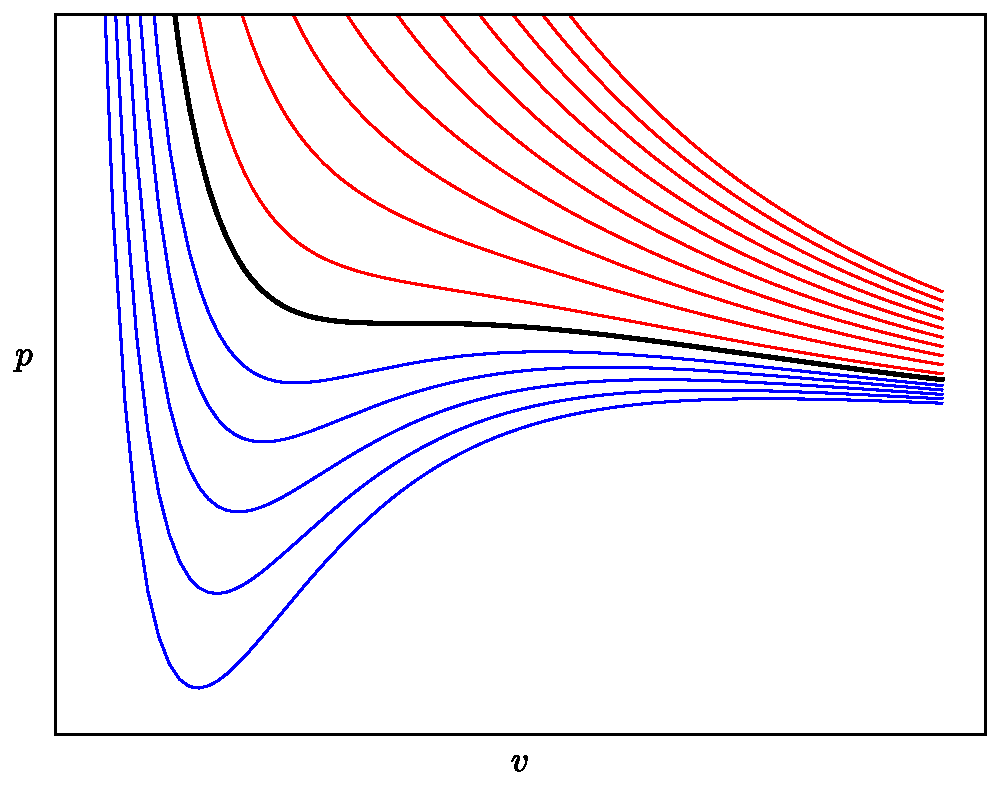
\includegraphics[width=0.75\textwidth]{Pseudopotential/vdW_isoth}
	\caption{Diagrama $p-v$ para la ecuaci\'on de van der Waals. Se destacan las isotermas supercr\'iticas (rojo), cr\'itica (negro) y subcr\'iticas (azul).}
	\label{fig:vdW_isoth}
\end{figure}

La \fig{fig:vdW_isoth} ejemplifica el comportamiento de la ecuaci\'on de van der Waals, donde cada l\'inea corresponde a una isoterma. A medida que la temperatura desciende, las isotermas pasan de un comportamiento similar a un gas ideal, en la esquina superior derecha de la figura, a exhibir un comportamiento en forma de S con un m\'inimo y un m\'aximo locales, en la esquina inferior izquierda. De acuerdo a esas isotermas, existen tres valores de densidad asociadas a una misma presi\'on. Sin embargo, en esa zona de S existe una regi\'on donde $(\partial v / \partial \rho)_T$ es positiva, y por lo tanto se tiene compresibilidad negativa, lo que implica que esa regi\'on es inestable frente a perturbaciones de presi\'on \cite{blundell_concepts_2006}.
La temperatura a partir de la cual se produce este cambio de comportamiento se conoce como temperatura cr\'tica, y es la que se ilustra con una l\'inea m\'as gruesa en la \fig{fig:vdW_isoth}. Esta isoterma presenta un punto de inflexi\'on, conocido como punto cr\'itico, sobre el que se definen propiedades caracter\'isticas de la ecuaci\'on de estado. En particular, analizando las derivadas $(\partial p / \partial v)_T = 0$ y $(\partial^2 p / \partial v^2)_T = 0$, puede encontrarse cu\'al es ese punto cr\'itico, es decir, los valores de presi\'on cr\'itica, volumen molar cr\'itico y temperatura cr\'itica que lo caracterizan:
\begin{equation}
	\begin{gathered}
		p_c = \dfrac{a}{27 b^2} \\
		v_c = 3b \\
		T_c = \dfrac{8 a}{27 R b}
	\end{gathered}
	\label{eq:vdw_param_crit}
\end{equation}

En la \fig{fig:vdW_isoth} se evidencia que para temperaturas por debajo del valor cr\'itico, dos vol\'umenes molares diferentes pueden adoptar el mismo valor de presi\'on en equilibrio $p_0$ (en realidad son 3, pero uno es inestable). Por lo tanto, puede establecerse un estado de coexistencia entre dos fases, l\'iquido y vapor, que compartan igual energ\'ia libre de Gibbs (o equivalentemente potencial qu\'imico). Esta restriccici\'on implica:
\begin{equation}
	\int_{v_l}^{v_g} \left[p_0 - p(v',T)\right] \, \mbox{d} v' = 0,
	\label{eq:maxwell_constr}
\end{equation}
donde $p_0 = p(v_l,T) = p(v_g,T)$. La \eq{eq:maxwell_constr} se conoce como regla de construcci\'on de Maxwell, y determina los vol\'umenes de coexistencia de ambas fases para una determinada temperatura. Si se realiza un cambio de variables adecuado, la \eq{eq:maxwell_constr} puede reescribirse como:
\begin{equation}
	\int_{\rho_g}^{\rho_l} \left[p_0 - p(\rho',T)\right] \dfrac{1}{\rho'} \, \mbox{d} \rho' = 0,
	\label{eq:maxwell_constr_rho}
\end{equation}
donde $p_0 = p(\rho_l,T) = p(\rho_g,T)$. Gr\'aficamente, resolver la regla de Maxwell implica encontrar los vol\'umenes para los que las \'areas sombreadas de la \fig{fig:vdW_Maxwell} sean iguales. 

\begin{figure}[ht]
	\centering
	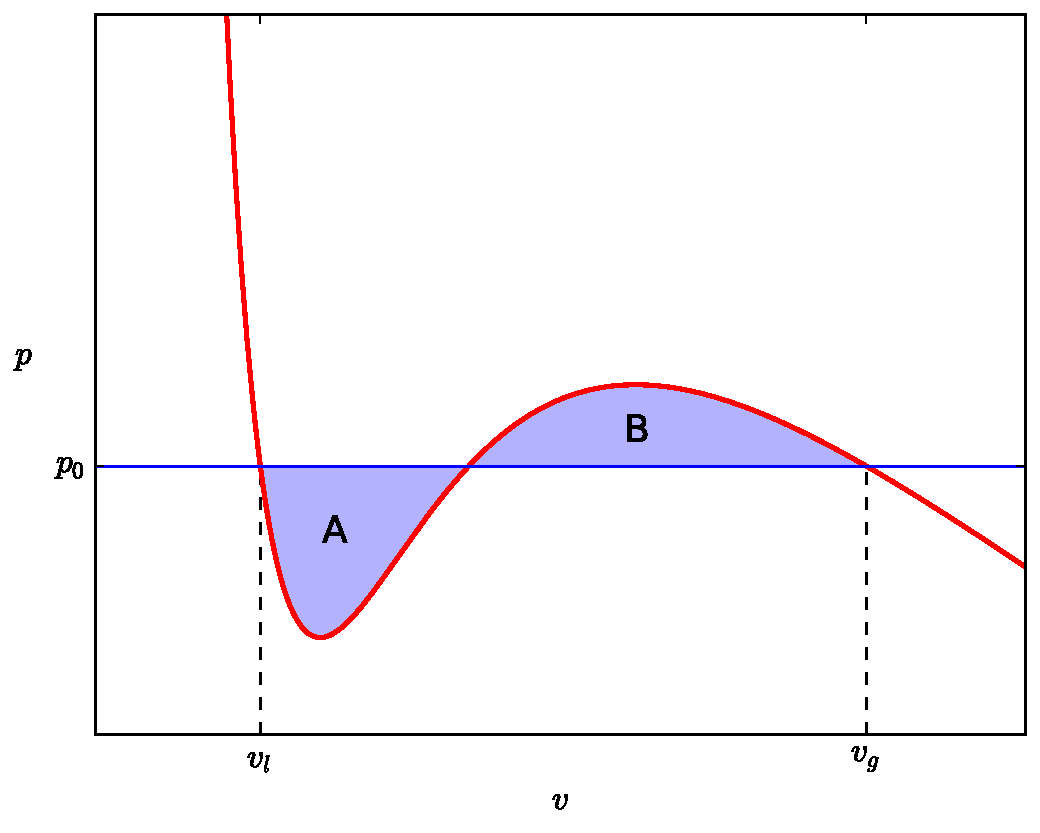
\includegraphics[width=0.75\textwidth]{Pseudopotential/vdW_Maxwell}
	\caption{Ejemplo de aplicaci\'on de la regla de construcci\'on de Maxwell. Dada una isoterma del diagrama $p-v$, los vol\'umenes de coexistencia son aquellos para los que las \'areas $A$ y $B$ son iguales.}
	\label{fig:vdW_Maxwell}
\end{figure}


La regla de construcci\'on de Maxwell aplica a cualquier ecuaci\'on de estado, e impone una restricci\'on termodin\'amica a las simulaciones realizadas con modelos pseudopotential: si se desea recuperar el comportamiento de un fluido regido por una ecuaci\'on de estado, entonces la ``separaci\'on autom\'atica de fases'' propia de esta familia debe ser capaz de reproducir las densidades de equilibrio dadas por la \eq{eq:maxwell_constr}.


\subsubsection*{Otras ecuaciones de estado}

La ecuaci\'on de estado de van der Waals ha alcanzado una notable popularidad, no s\'olo por ser la primera en modelar el comportamiento de gases reales, sino porque a pesar de su simplicidad, permite representar fen\'omenos complejos asociados a la coexistencia y cambio de fase. Sin embargo, esta ecuaci\'on no es la \'unica, ya que se ha creado un amplio abanico de posibilidades en busca de una mejor representaci\'on de diversos tipos de fluidos. A continuaci\'on se detallan dos de las m\'as conocidas, apliamente utilizadas en la literatura de lattice Boltzmann.

\smallskip
\textbf{Carnahan-Starling:}
\begin{equation}
	\begin{gathered}
		p = \rho R T\dfrac{1+b\rho/4+(b\rho/4)^2-(b\rho/4)^3}{(1-b\rho/4)^3} - a\rho^2, \\[2mm]
		p_c = \dfrac{0.07066 \, Ra}{b^2}, \\[2mm]
		T_c = \dfrac{0.37733 \, a}{Rb}, \\[2mm]
		\rho_c = \dfrac{0.5218}{b}
	\end{gathered}
\end{equation}


\textbf{Peng-Robinson:}
\begin{equation}
	\begin{gathered}
		p = \dfrac{\rho R T}{1-b\rho} - \dfrac{a\varphi(\omega,T)\rho^2}{1+2b\rho-(b\rho)^2}, \\[0mm]
		\varphi(\omega,T) = \left[ 1+(0.37464+1.54226\omega-0.26992\omega^2)(1-\sqrt{T/T_c})\right], \\[0mm]
		p_c \approx \dfrac{0.01324 \, a}{b^2}, \\[2mm]
		T_c \approx \dfrac{0.17015 \, a}{Rb}, \\[2mm]
		\rho_c \approx \dfrac{0.253077}{b}
	\end{gathered}
\end{equation}

\red{Poner ac\'a otras propiedades derivadas, como calor latente?}


\subsubsection*{Curvas de coexistencia}

Como se mencion\'o previamente, la regla de construcci\'on de Maxwell permite determinar las densidades de coexistencia en equilibrio para cualquier ecuaci\'on de estado. La determinaci\'on de los l\'imites de esta integral no siempre es sencillo, dado que requiere la aplicaci\'on de un ciclo iterativo, con resultads que dependen de las constantes caracter\'isticas de cada ecuaci\'on de estado. Este c\'alculo, as\'i como la comparaci\'on objetiva entre diferentes ecuaciones de estado, puede simplificarse si se usa el concepto de unidades reducidas \cite{mcquarrie_molecular_1999}:
\begin{equation}
	\rho_r = \rho / \rho_c, \qquad T_r = T / T_c, \qquad p_r = p / p_c,
\end{equation}
donde los sub\'indices $r$ y $c$ denotan propiedades reducidas y cr\'iticas, respectivamente. De acuerdo a la ley de estados correspondientes, las propiedades reducidas deben ser las mismas independientemente del tipo de unidades utilizadas. Por lo tanto, la relaci\'on entre propiedades de coexistencia quedan un\'ivocamente determinadas para cada ecuaci\'on de estado, si se emplean unidades reducidas. De esta forma pueden construirse las llamadas curvas universales de coexistencia, como las mostradas en la \fig{fig:EOS}.

\begin{figure}[ht]
	\centering
	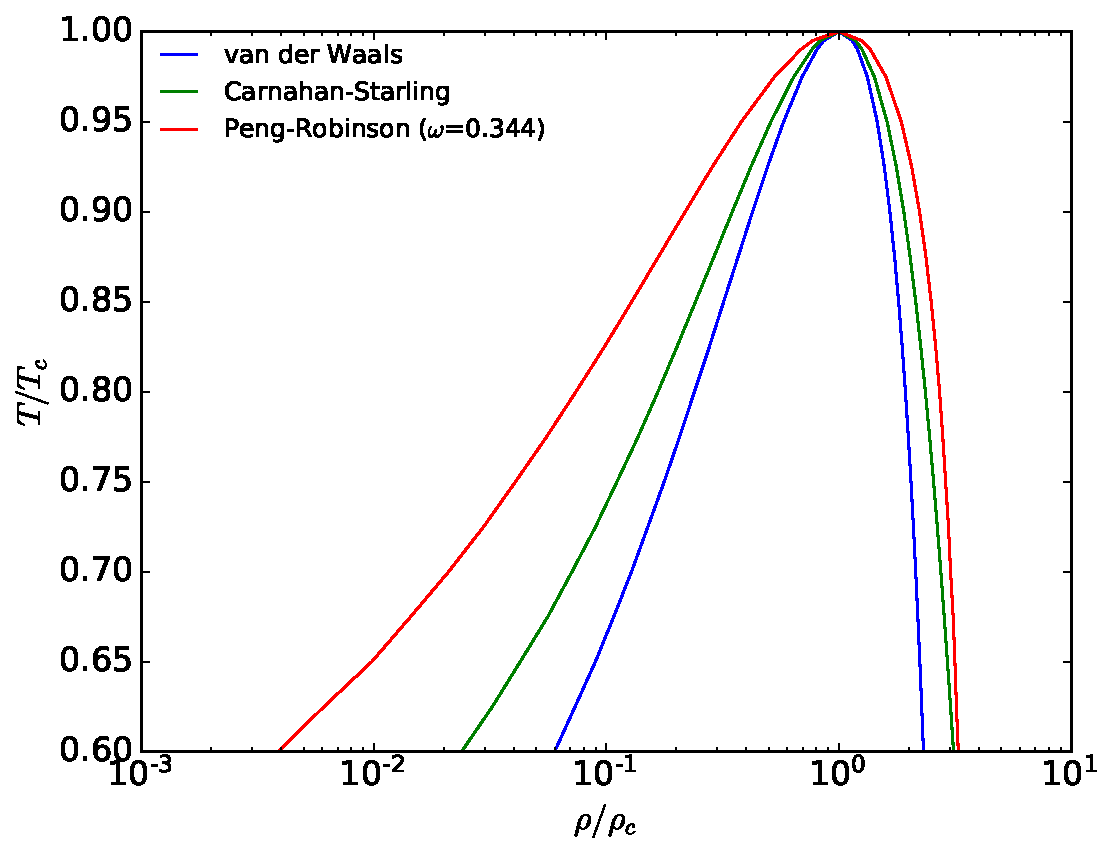
\includegraphics[width=0.75\textwidth]{Pseudopotential/EOS_comp}
	\caption{Densidades de coexistencia, en unidades reducidas, para diferentes ecuaciones de estado.}
	\label{fig:EOS}
\end{figure}





\subsection{Incorporaci\'on de ecuaciones de estado en el potencial de interacci\'on}

La definici\'on de masa efectiva dada por Shan y Chen se aproxima a un valor asint\'otico cuando la densidad es alta, lo que contribuye a evitar el colapso de la fase de mayor densidad y, por lo tanto, contribuir a mejorar la estabilidad de las simulaciones. Sin embargo, el uso de esta expresi\'on fija la ecuaci\'on de estado final, lo que limita la aplicabilidad a diferentes fluidos. En 2006. Yuan y Schaefer \cite{yuan_equations_2006} demostraron que es posible alcanzar relaciones de densidad elevadas en casos est\'aticos si se emplea la masa efectiva introducida por He y Doolen \cite{he_thermodynamic_2002}:
\begin{equation}
	\psi(\rho) = \sqrt{\dfrac{2(p_{EOS} - \rho c_s^2)}{Gc^2}},
	\label{eq:potencial}
\end{equation}
donde $p_{EOS}$ representa una ecuaci\'on de estado no ideal, como Van der Waals, Carnahan-Starling o Peng-Robinson.


\subsection{\red{Adicionales?}}

\red{Podr\'ian ponerse ac\'a ciertos t\'opicos, como la recuperaci\'on de la tensi\'on superficial}






\subsection{La condici\'on de estabilidad mec\'anica y el problema de inconsistencia termodn\'amica}

En el caso sin fuerzas de interacci\'on, a nivel macrosc\'opico se recupera una ecuaci\'on de estado ideal de la forma $p=\rho c_s^2$. Sin embargo, la incorporaci\'on de \ref{eq:f_int} produce una nueva ecuaci\'on de estado dependiente del potencial de interacci\'on:
\begin{equation}
	p = \rho c_s^2 + \dfrac{G}{2} c_s^2 \psi ^2,
\end{equation}
mientras que el tensor de presi\'on $\bm{P}$ queda definido como \cite{he_thermodynamic_2002}:
\begin{equation}
	\nabla \cdot \bm{P} = \nabla \cdot (\rho c_s^2 \bm{I}) - \bm{F}.
	\label{eq:ptens}
\end{equation}

Shan \cite{shan_pressure_2008} demostr\'o que para garantizar un balance mec\'anico exacto, debe considerarse una forma discreta del tensor de presi\'on. En particular, esta expresi\'on puede derivarse a partir de una integral de volumen de la \eq{eq:ptens}:
\begin{equation}
	\int (\nabla \cdot \bm{P}) \, \mbox{d}\Omega = \int \nabla \cdot (\rho c_s^2 \bm{I})\, \mbox{d}\Omega - \int \bm{F} \, \mbox{d}\Omega,
	\label{eq:integral_pres}
\end{equation}
donde $\Omega$ es un volumen cerrado. Si se aplica el teorema de integraci\'on de Gauss a la \eq{eq:integral_pres} resulta
\begin{equation}
	\int \bm{P} \, \mbox{d} \bm{A} = \int \rho c_s^2 \bm{I}\, \mbox{d} \bm{A} - \int \bm{F} \, \mbox{d}\Omega,
\end{equation}
donde $\mbox{d} \bm{A}$ es un diferencial de \'area. En forma discreta, esta integral puede escribirse como
\begin{equation}
	\sum \bm{P} \cdot \bm{A} = \sum \rho c_s^2 \bm{I} \cdot \bm{A} - \sum \bm{F}.
\end{equation}

Por lo tanto, el tensor de presi\'on finalmente puede escribirse como:
\begin{equation}
	\bm{P} = \rho c_s^2 \bm{I} + \dfrac{G}{2}\psi(\bm{x}) \sum_{\alpha=1}^N w(|\bm{e}_{\alpha}|^2)\psi(\bm{x}+\bm{e}_{\alpha})\bm{e}_{\alpha}\bm{e}_{\alpha}.
	\label{eq:ptens_shan}
\end{equation}

En el caso de considerar s\'olo interacciones con los vecinos cercanos (ubicados a una distancia m\'axima de $\sqrt{2}$ o $\sqrt{3}$ unidades de grilla en 2 o 3 dimensiones respectivamente), la expansi\'on en serie de Taylor de la \eq{eq:ptens_shan} resulta:
\begin{equation}
	\bm{P} = \left( \rho c_s^2 + \dfrac{G c^2}{2} \psi^2 + \dfrac{G c^4}{12} \psi \nabla^2 \psi \right) \bm{I} + \dfrac{G c^4}{6} \psi \nabla \nabla \psi.
	\label{eq:ptens_shan_taylor}	
\end{equation}

La \eq{eq:ptens_shan_taylor} puede usarse para determinar la presi\'on normal a una interfase plana
\begin{equation}
	P_n = \rho c_s^2 + \dfrac{G c^2}{2} \psi^2 + \dfrac{G c^4}{12} \left[ \alpha \left( \dfrac{d\psi}{dn} \right)^2 + \beta \psi \dfrac{d^2 \psi}{dn^2} \right],
	\label{eq:ptens_shan_plane}	
\end{equation}
donde $n$ denota la direcci\'on normal a la interfase, y en el caso de interacci\'on de vecinos cercanos se cumple $\alpha = 0$ y $\beta = 3$. Por lo tanto, tomando como base la \eq{eq:ptens_shan_plane} y considerando que en equilibrio la presi\'on $P_n$ debe ser igual a la presi\'on est\'atica en el seno del fluido \cite{shan_pressure_2008}, puede derivarse la condici\'on de estabilidad mec\'anica:
\begin{equation}
	\int_{\rho_g}^{\rho_l} \left( p_0 - \rho c_s^2 - \dfrac{Gc^2}{2} \psi^2 \right) \dfrac{\psi'}{\psi^{1+\varepsilon}} \, \mbox{d}\rho = 0,
\end{equation}
donde $\psi' = d\psi / d\rho$, $\varepsilon=-2\alpha/\beta$ y $p_0=p(\rho_l)=p(\rho_g)$. De esta forma, puede verse que la condici\'on de estabilidad mec\'anica conduce a densidades de coexistencia que en general ser\'an diferentes a las establecidas por la construcci\'on de Maxwell (\eq{eq:maxwell_constr_rho}), ya que si el potencial de interacci\'on satisface la propuesta de He y Doolen, entonces en general no puede cumplirse que $\psi' / \psi^{1+\varepsilon} \propto 1/\rho^2$. Esta incompatibilidad se conoce con el nombre de inconsistencia termodin\'amica.


\section{El modelo isot\'ermico de Li et al.}

Los modelos pseudopotential proveen una alternativa sencilla y eficiente para poder simular num\'ericamente el comportamiento de flujos m\'ultif\'asicos. Esta simplicidad, sin embargo, tiene su precio: las primeras versiones encontraron r\'apidamente un l\'imite de aplicabilidad, no s\'olo por el problema de inconsistencia termodin\'amica, sino por la fuerte presencia de corrientes esp\'ureas en las interfases, a\'un en problemas est\'aticos o cuasi-est\'aticos. Esta combinaci\'on de factores llev\'o a que durante mucho tiempo, el uso del m\'etodo pseudopotential se limitase a la resoluci\'on de problemas con baja relaci\'on de densidades y bajo n\'umero de Reynolds.

El camino hacia versiones m\'as estables fue forj\'andose con trabajos que buscan identificar el origen de estas inestabilidades num\'ericas, junto con mecanismos te\'oricos para remediarlas (al menos parcialmente). A modo de ejemplo es interesante destacar el trabajo de Shan \cite{shan_analysis_2006}, en el cu\'al se describe a las corrientes esp\'ureas como un fen\'omeno que tiene lugar cerca de la interfase de una burbuja estacionaria, y en el cual se produce un flujo peque\~no pero finito alrededor de la misma. El patr\'on de este flujo presenta la misma simetr\'ia que la grilla subyacente, y su magnitud es inversamente proporcional a la viscosidad del fluido simulado. Shan demostr\'o que existe una conexi\'on directa entre este fen\'omeno y la falta de isotrop\'ia en ciertos operadores diferenciales discretos, en particular el empleado en la reprentaci\'on discreta de la fuerza de interacci\'on (\eq{eq:f_int}). Denotando a los tensores 
\begin{equation}
	E^{(n)}_{i_1i_2\ldots i_n} = \sum_{\alpha}w(|\bm{e}_{\alpha}|^2)(\bm{e}_{\alpha})_{i_1} \cdots (\bm{e}_{\alpha})_{i_n},
\end{equation}
entonces puede escribirse el gradiente de una funci\'on $f$ como:
\begin{equation}
	\sum_{\alpha}w(|\bm{e}_{\alpha}|^2) f(\bm{x}+\bm{e}_{\alpha})\bm{e}_{\alpha}=(\nabla f)\cdot \bm{E}^{(2)} + \dfrac{1}{3!}(\nabla^{(3)} f)\cdot \bm{E}^{(4)} + \dfrac{1}{5!}\nabla^{(5)} f)\cdot \bm{E}^{(6)} + \ldots.
\end{equation}
Por lo tanto, la mejor aproximaci\'on a $\nabla f$ se logra si todos los tensores $\bm{E}^{(n)}$ son isotr\'opicos, aunque este requisito no puede alcanzarse debido a que existe un n\'umero finito de  velocidades discretas. Sin embargo, Shan demostr\'o que pueden encontrarse conjuntos adecuados de pesos $\{ w(\bm{e}_{\alpha})\}$ que mejoran notoriamente la isotrop\'ia de la aproximaci\'on, y por lo tanto, reducen la magnitud de las corrientes esp\'ureas.

Dentro de un contexto similar al presentado por Shan, Sbragaglia y sus colaboradores adoptaron una nueva expresi\'on para la fuerza de interacci\'on en la que se tienen en cuenta las interacciones de rango medio, es decir, se consideran aquellos nodos que no son vecinos inmediatos \cite{sbragaglia_generalized_2007}:
\begin{equation}
	\bm{F}_i = -c_s^2 \psi(\bm{x}) \sum_{\alpha} w(|\ea|^2) \left[G_1 \psi(\xplus)  + G_2 \psi(\bm{x}+2\bm{e}_{\alpha}) \right]
	\label{eq:fi_sbragaglia}
\end{equation}

Usando esta aproximaci\'on, Sbragaglia et al. demostraron anal\'iticamente que, para una interfase plana, la \eq{eq:fi_sbragaglia} conduce a una tensi\'on superficial que depende de las constantes $G_1$ y $G_2$, y por lo tanto es ajustable. Por otro lado, la extensi\'on del stencil en el c\'alculo de la fuerza de interacci\'on permite reducir el espesor de la interfase y elevar la relaci\'on de densidades en simulaciones estacionarias.

\red{poner cambios en esquemas de fuerzas}

Las contribuciones de Shan y Sbragaglia ilustran la evoluci\'on que ha sufrido (y que contin\'ua experimentando) el modelo original de Shan y Chen buscando mejorar la precisi\'on, estabilidad y aplicabilidad del m\'etodo. En pocas palabras, estos esfuerzos pueden describirse como un compromiso entre la aplicaci\'on adecuada de la fuerza de interacci\'on, y la preservaci\'on de un algoritmo eficiente y de sencilla implementaci\'on.

\red{Mencionar que son modelos 2D}
Entre las alternativas pseudopotential m\'as recientes, el modelo introducido por Li et al. \cite{li_lattice_2013} contiene esas caracter\'isticas de equilibrio antes mencionadas. En esta propuesta se hace uso de un operador de colisi\'on MRT, de modo que la \lbe{} vectorial resulta:
\begin{equation}
	\bm{f} (\bm{x} + \bm{e}\delta_t, t+\delta_t) = \bm{M}^{-1}\left[ \bm{m} - \bm{\Lambda}(\bm{m} - \feq{m})  + \delta_t \left( \bm{I} - \dfrac{\bm{\Lambda}}{2} \bar{\bm{S}} \right) \right].
	\label{eq:lbe_li}
\end{equation}

Como se mostr\'o en el \red{Cap\'itulo 2}, $\bm{m} = \bm{Mf}$ corresponde a la proyecci\'on de la funci\'on de distribuci\'on $\bm{f}$ en el espacio de momentos, y $\feq{m} = \bm{M}\feq{f}$ a la transformaci\'on de la distribuci\'on de equilibrio. En este caso se usa la matriz de transformaci\'on y funci\'on de equilibrio est\'andar (\red{Ecuaciones XX y YY respectivamente}), de modo que la distribuci\'on de equilibrio en el espacio de momentos puede escribirse como:
\begin{equation}
\feq{m} = \rho (1, -2+3|\bm{u}|^2, 1-3|\bm{u}|^2, u_x, -u_x, u_y, -u_y, u_x^2-u_y^2, u_xu_y)^T.
\end{equation}

La matriz $\bm{\Lambda}$ corresponde a una matriz diagonal cuyos componentes se denotan mediante
\begin{equation}
	\bm{\Lambda}=diag(\tau_{\rho}^{-1},\tau_{e}^{-1},\tau_{\zeta}^{-1},\tau_{j}^{-1},\tau_{q}^{-1},\tau_{j}^{-1},\tau_{q}^{-1},\tau_{\nu}^{-1},\tau_{\nu}^{-1}).
\end{equation}

En este modelo, las cantidades macrosc\'opicas conservadas corresponden a la densidad y velocidad, y pueden recuperarse siguiendo el esquema de fuerzas de Guo:
\begin{equation}
	\begin{gathered}
		\rho = \sum_{\alpha} f_{\alpha}, \\
		\rho \bm{u} = \sum_{\alpha} \bm{e}_{\alpha} f_{\alpha} + \dfrac{\delta_t}{2} \bm{F},
	\end{gathered}
\end{equation}

donde $\bm{F}$ corresponde a la fuerza total actuando sobre el sistema. En la mayor\'ia de los casos analizados, $\bm{F}$ contiene una componente volum\'etrica ($\bm{F}_b$) y otra asociada al potencial de interacci\'on, de modo que se utiliza $\bm{F} = \bm{F}_b + \bm{F}_i$.

Siguiendo la idea detallada en un trabajo anterior de Li y sus colaboradores \cite{li_forcing_2012}, la fuerza de interacci\'on tambi\'en debe incorporarse durante la colisi\'on a trav\'es del t\'ermino de fuente $\bar{\bm{S}}$, definido en el espacio de momento como:
\begin{equation}
 \bar{\bm{S}} = 
 \left[ 
 	\begin{array}{c} 
 		0	\\
 		6 \bm{u} \cdot \bm{F} + \dfrac{12\sigma |\bm{F}_i|^2}{\psi^2 \delta_t (\tau_e-0.5)} \\
 		-6 \bm{u} \cdot \bm{F} - \dfrac{12\sigma |\bm{F}_i|^2}{\psi^2 \delta_t (\tau_{\zeta}-0.5)} \\
 		F_x \\
 		-F_x \\
 		F_y \\
 		-F_y \\
 		2(u_xF_x - u_yF_y) \\
 		(u_xF_y + u_yF_x)
 	\end{array} 
 \right]
 \label{eq:s_li}
\end{equation}

La principal novedad del modelo de Li consiste en la incorporaci\'on de t\'erminos adicionales en las componentes 1 y 2 de la \eq{eq:s_li}, que dependen linealmente de un par\'ametro libre $\sigma$. En particular, aplicando la expansi\'on de Chapman-Enskog a las Ecs.~(\ref{eq:lbe_li})-(\ref{eq:s_li}) se demuestra que las variables macrosc\'opicas satisfacen:
\begin{equation}
	\dfrac{\partial (\rho \bm{u})}{\partial t} + \nabla \cdot (\rho \bm{uu}) = -\nabla \cdot (\rho c_s^2 \bm{I}) + \nabla \cdot \bm{\Pi} + \bm{F} - 2G^2 c^4 \sigma \nabla \cdot (|\nabla \psi|^2 \bm{I}),
	\label{eq:li_macro}
\end{equation}
de modo que el nuevo tensor de presi\'on satisface:
\begin{equation}
	\nabla \cdot \bm{P} = \nabla \cdot (\rho c_s^2 \bm{I}) - \bm{F} + 2G^2 c^4 \sigma \nabla \cdot (|\nabla \psi|^2 \bm{I})
\end{equation}
y, de acuerdo a la metodolog\'ia de Shan \cite{shan_pressure_2008}, puede escribirse como:
\begin{equation}
	\bm{P} = \bm{P}_{\mbox{orig}} + 2G^2 c^4 \sigma (|\nabla \psi|^2 \bm{I}),
\end{equation}
donde $\bm{P}_{\mbox{orig}}$ corresponde al tensor original definido por la \eq{eq:ptens_shan_taylor}. De este resultado se desprende que la nueva diferencia de presi\'on a trav\'es de una interfase plana corresponde a:
\begin{equation}
	P_n = \rho c_s^2 + \dfrac{G c^2}{2} \psi^2 + \dfrac{G c^4}{12} \left[ (\alpha+24G\sigma) \left( \dfrac{d\psi}{dn} \right)^2 + \beta \psi \dfrac{d^2 \psi}{dn^2} \right],
\end{equation}
y, por lo tanto, $\varepsilon=-2(\alpha + 24 G \sigma)/\beta$. De esta manera, la condici\'on de estabilidad mec\'anica ($\varepsilon$) ya no queda determinada s\'olo por el conjunto de velocidades de grilla, sino que puede ajustarse a trav\'es del par\'ametro libre $\sigma$. Esta nueva aproximaci\'on sigue sin cumplir formalmente con la incompatibilidad planteada por la inconsistencia termodin\'amica, pero como se muestra en las secciones siguientes, permite alcanzar una excelente representaci\'on de las curvas de coexistencia para un amplio rango de temperaturas.


\section{Validaci\'on}

El modelo isot\'ermico de Li ha sido utilizado exitosamente en la simulaci\'on de problemas multif\'asicos diversos, como el impacto de droplets sobre una superficie plana o en la medici\'on de frecuencia de escilaci\'on de droplets aislados. Por lo tanto, para el desarrollo de esta tesis se continu\'o con la evaluaci\'on de problemas num\'ericos que permiten reproducir fen\'omenos caracter\'isticos de flujos complejos, a la vez que aporten una caracterizaci\'on efectiva de LB como m\'etodo num\'erico.

\subsection{Construcci\'on de Maxwell}

La inconsistencia termodin\'amica intr\'inseca de los modelos \pp{} obliga a llevar a cabo, como primer paso de verificaci\'on, experimentos num\'ericos destinados a cuantificar la desviaci\'on entre las densidades de coexistencia reproducidas por el modelo y aquellas definidas mediante la regla de construcci\'on de Maxwell. Estos experimentos, conocidos simplemente como de construcci\'on de Maxwell, consisten b\'asicamente en la simulaci\'on de un sistema adecuado, simple, pero que a la vez involucre la fenomenolog\'ia buscada.

En este caso, el problema elegido consiste en la simulaci\'on de una regi\'on bidimensional con condiciones de contorno peri\'odicas, temperatura uniforme, sin fuerzas externas, y que inicialmente contiene un fluido con densidad perturbada aleatoriamente en  $\pm 1\%$ alrededor del valor cr\'itico ($\rho=\rho_c$). Como se ejemplifica en la \fig{fig:maxwell_2d}, en los primeros instantes de simulaci\'on comienzan a generarse regiones de diferente densidad, que contin\'uan separ\'andose y agrup\'andose hasta formar estructuras estacionarias, con densidades claramente diferentes. De esta manera, pueden tomarse los valores de densidad en el interior de cada fase, lejos de las interfases, y compararlos con los determinados por la regla de Maxwell.

\begin{figure}[htb]
    \centering
    \begin{subfigure}[t]{0.45\textwidth}
        \centering
        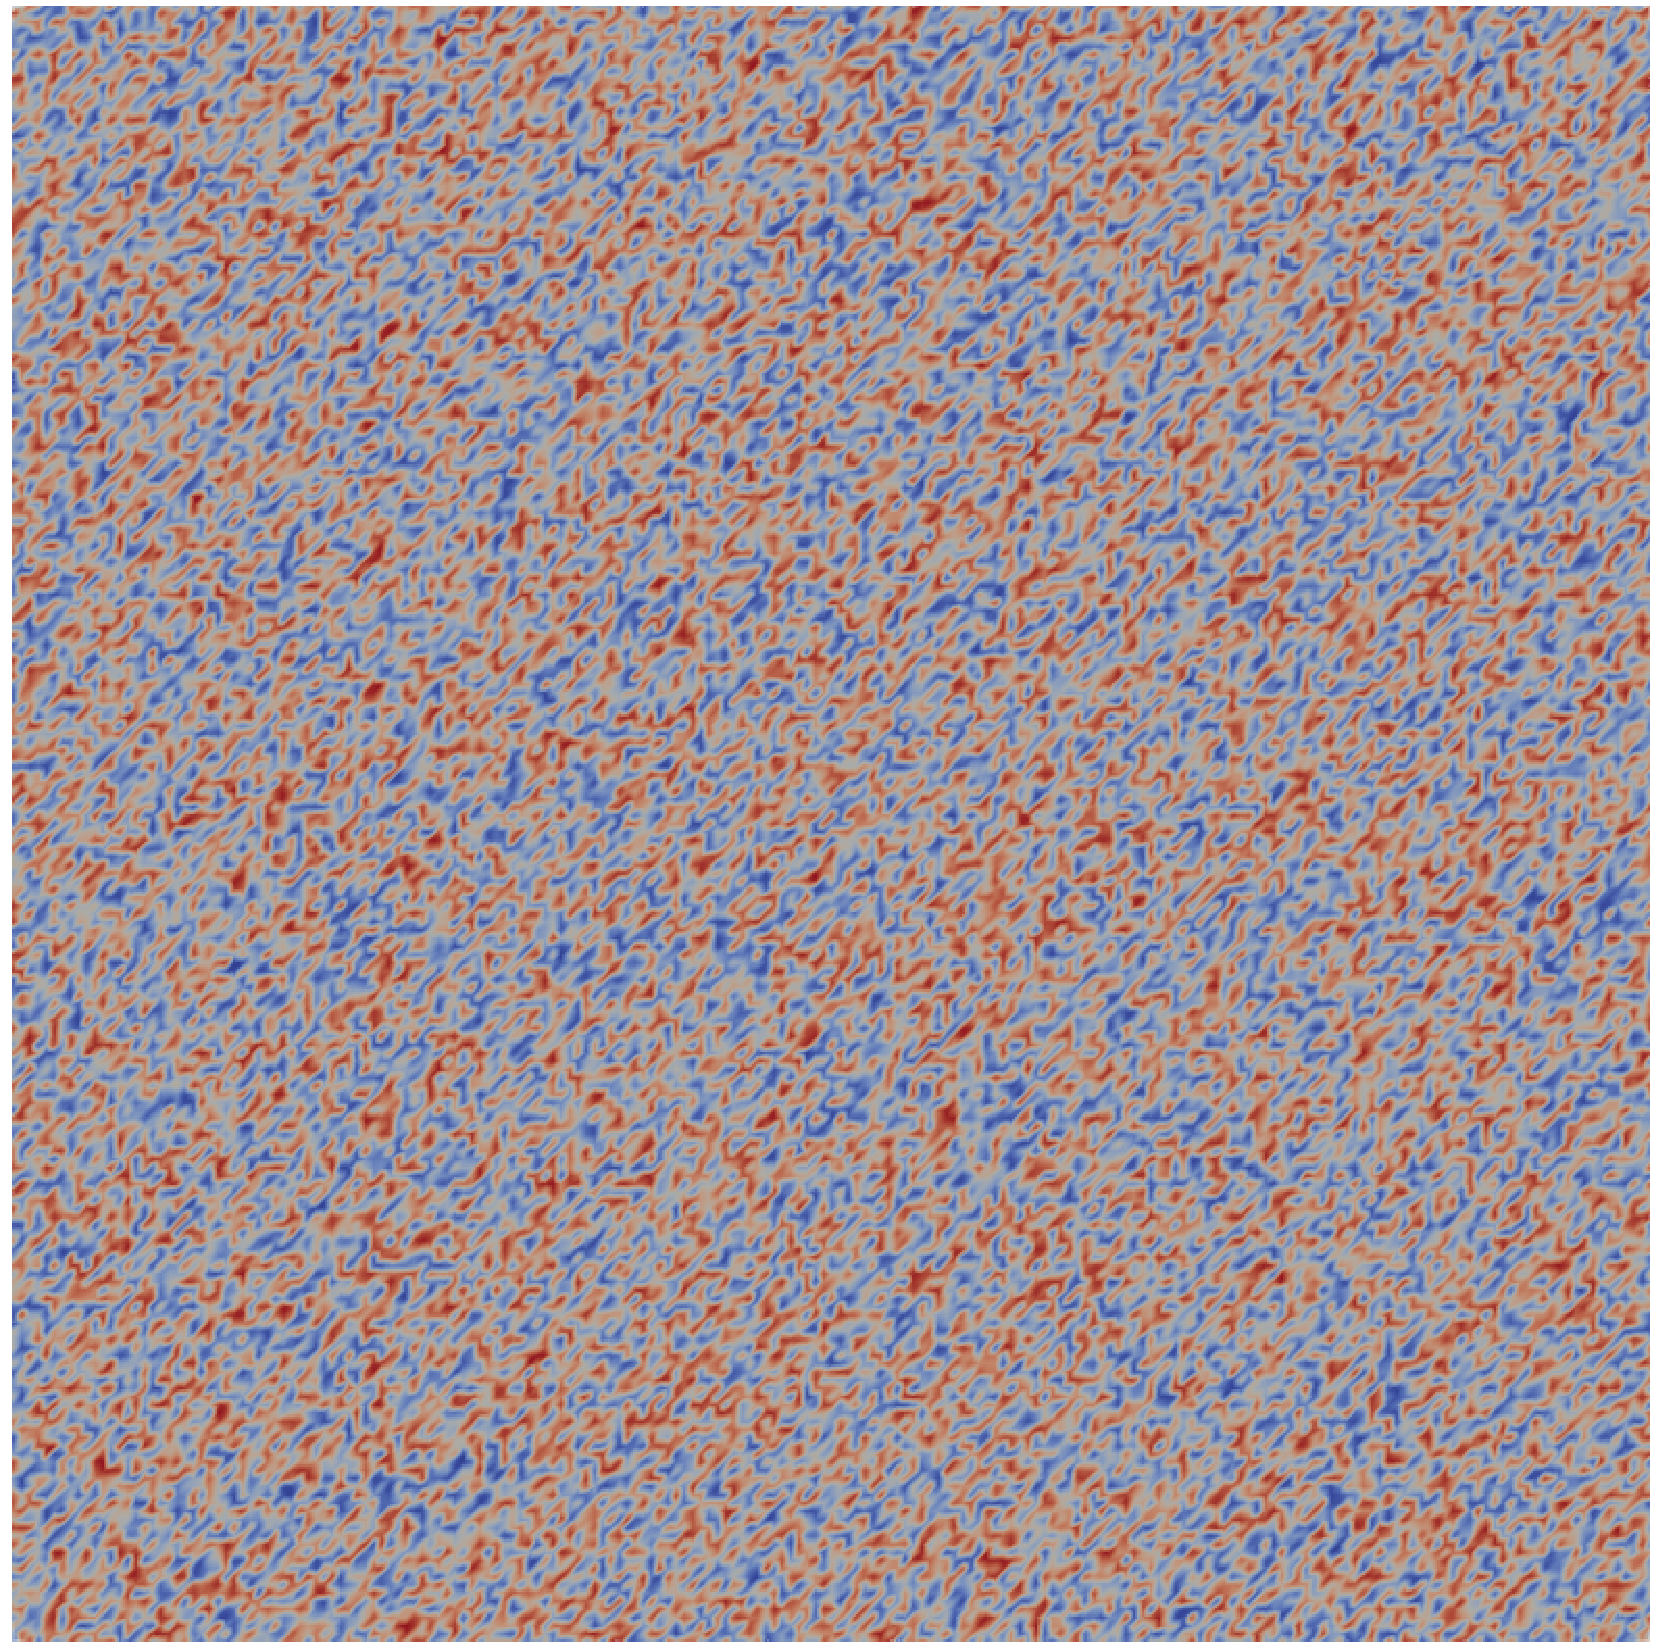
\includegraphics[width=0.95\textwidth]{Imagenes/Maxwell2D/Maxwell2D_sim/Imagenes/t_0}
        \caption{$t=0$}
    \end{subfigure}
    \begin{subfigure}[t]{0.45\textwidth}
        \centering
        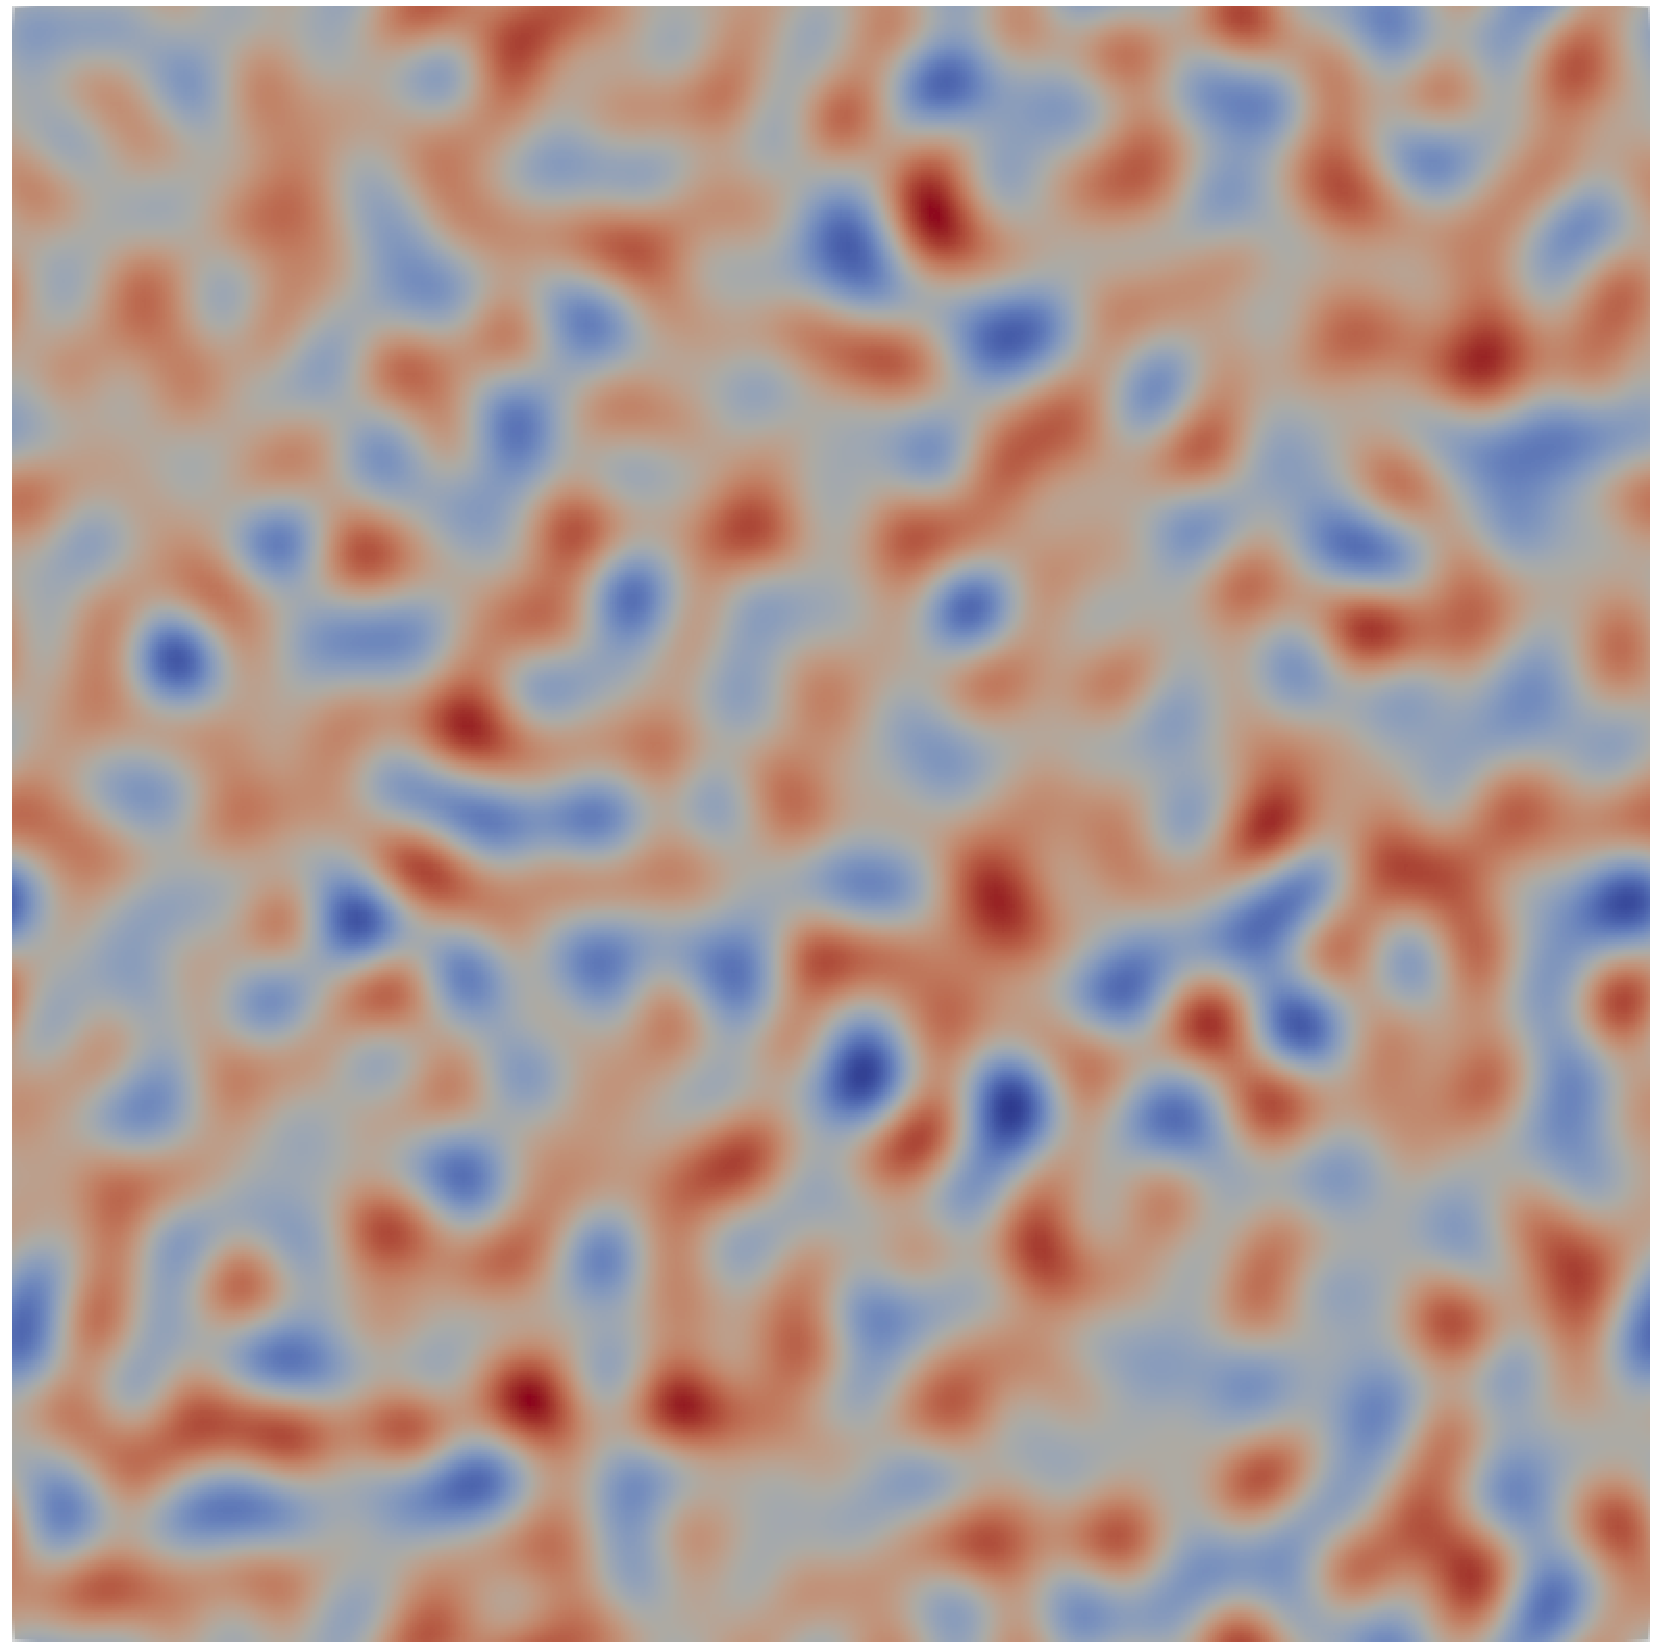
\includegraphics[width=0.95\textwidth]{Imagenes/Maxwell2D/Maxwell2D_sim/Imagenes/t_50}
        \caption{$t = 50$}
    \end{subfigure}
    \begin{subfigure}[t]{0.45\textwidth}
        \centering
        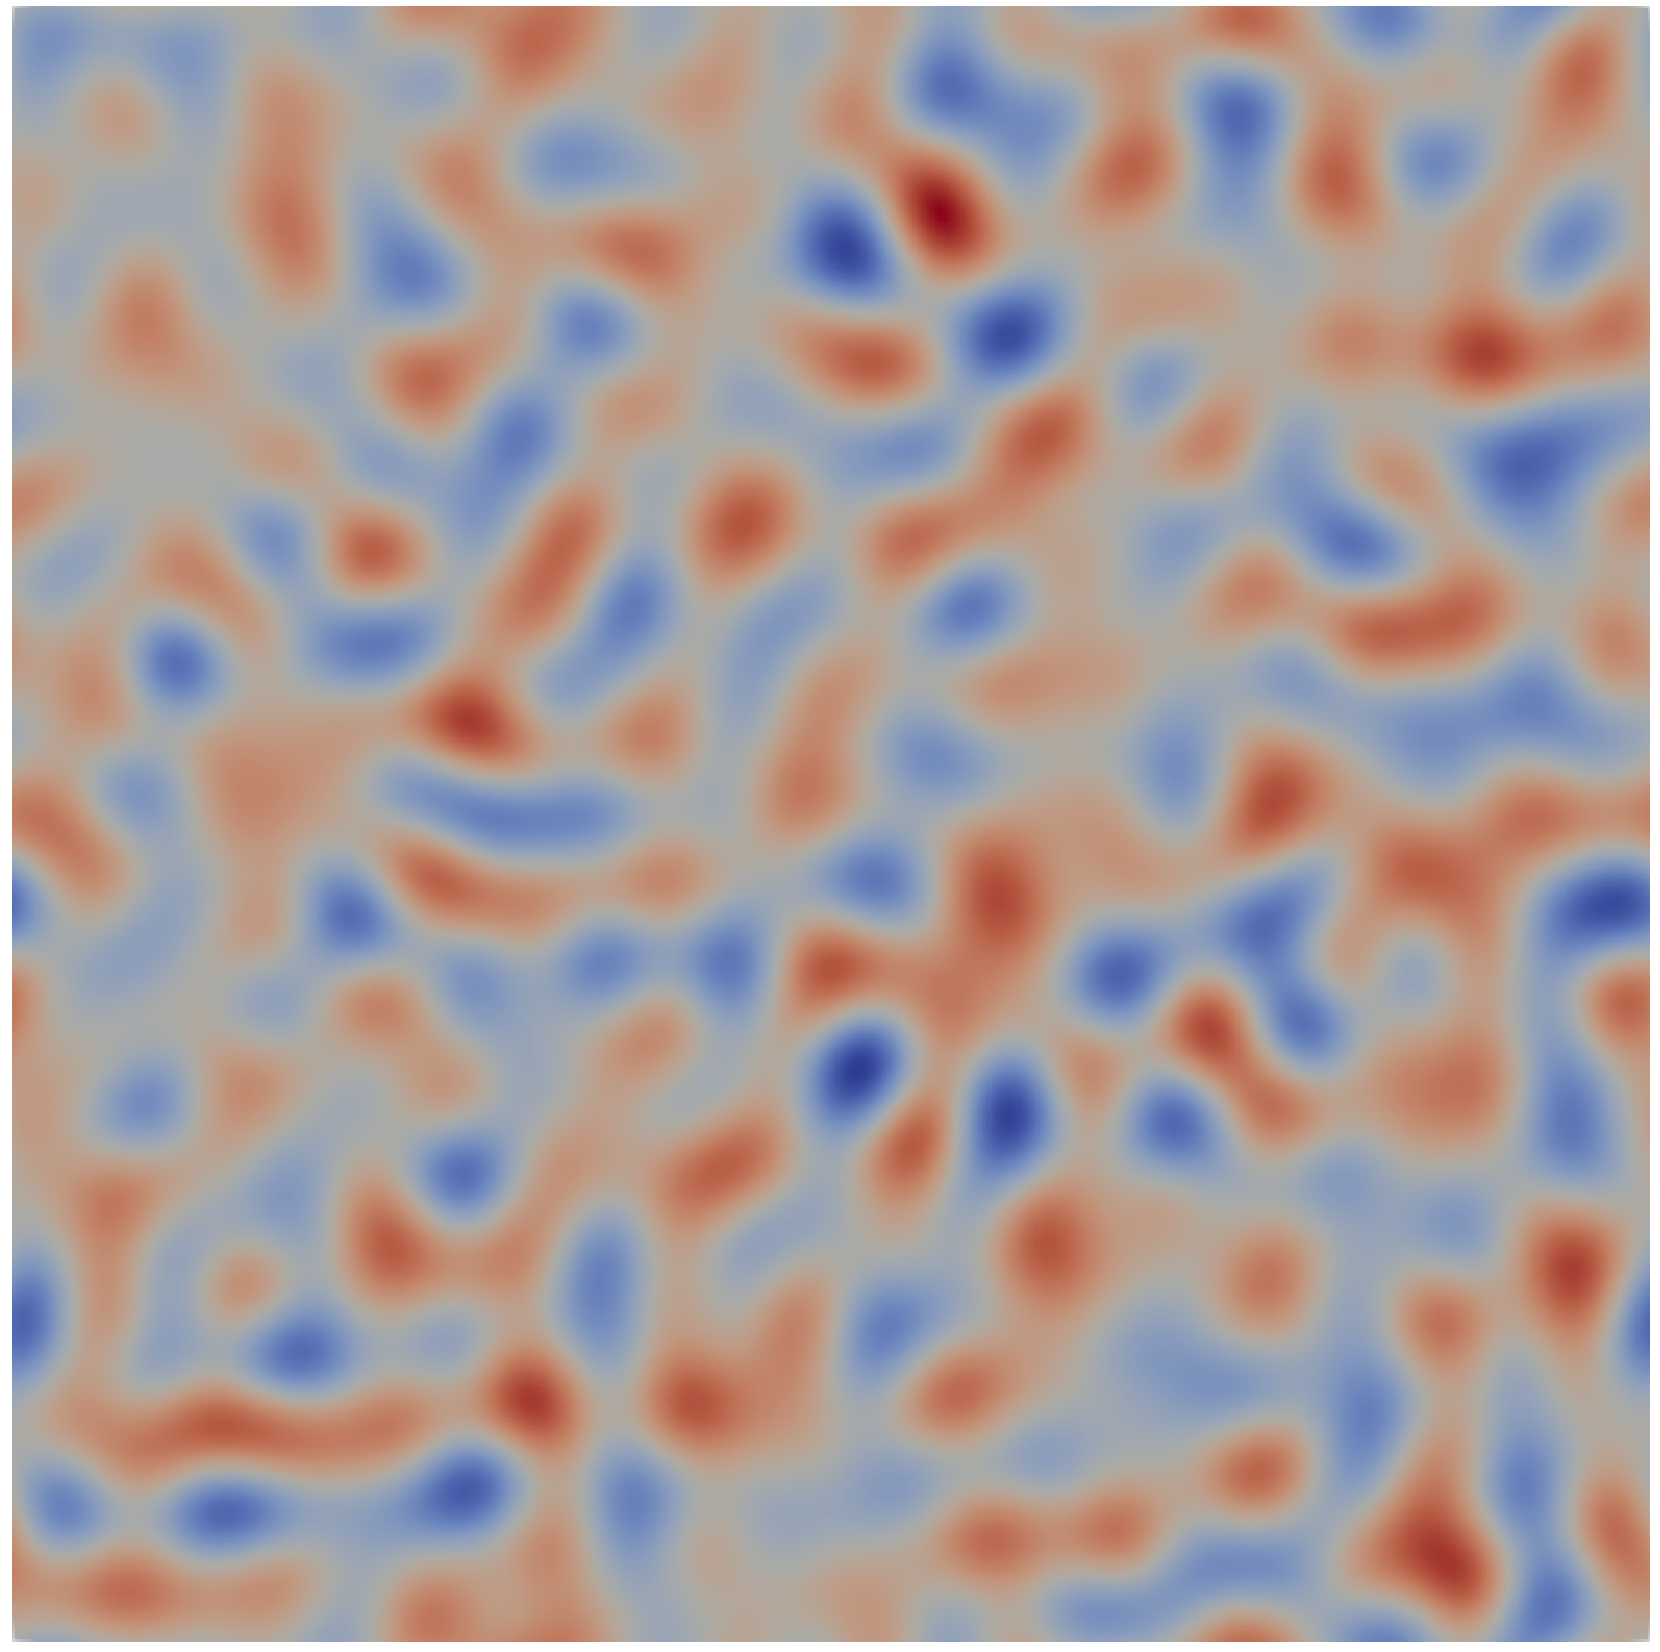
\includegraphics[width=0.95\textwidth]{Imagenes/Maxwell2D/Maxwell2D_sim/Imagenes/t_100}
        \caption{$t = 100$}
    \end{subfigure}    
    \begin{subfigure}[t]{0.45\textwidth}
        \centering
        \includegraphics[width=0.95\textwidth]{Imagenes/Maxwell2D/Maxwell2D_sim/Imagenes/t_500}
        \caption{$t = 500$}
    \end{subfigure}    
    \begin{subfigure}[t]{0.45\textwidth}
        \centering
        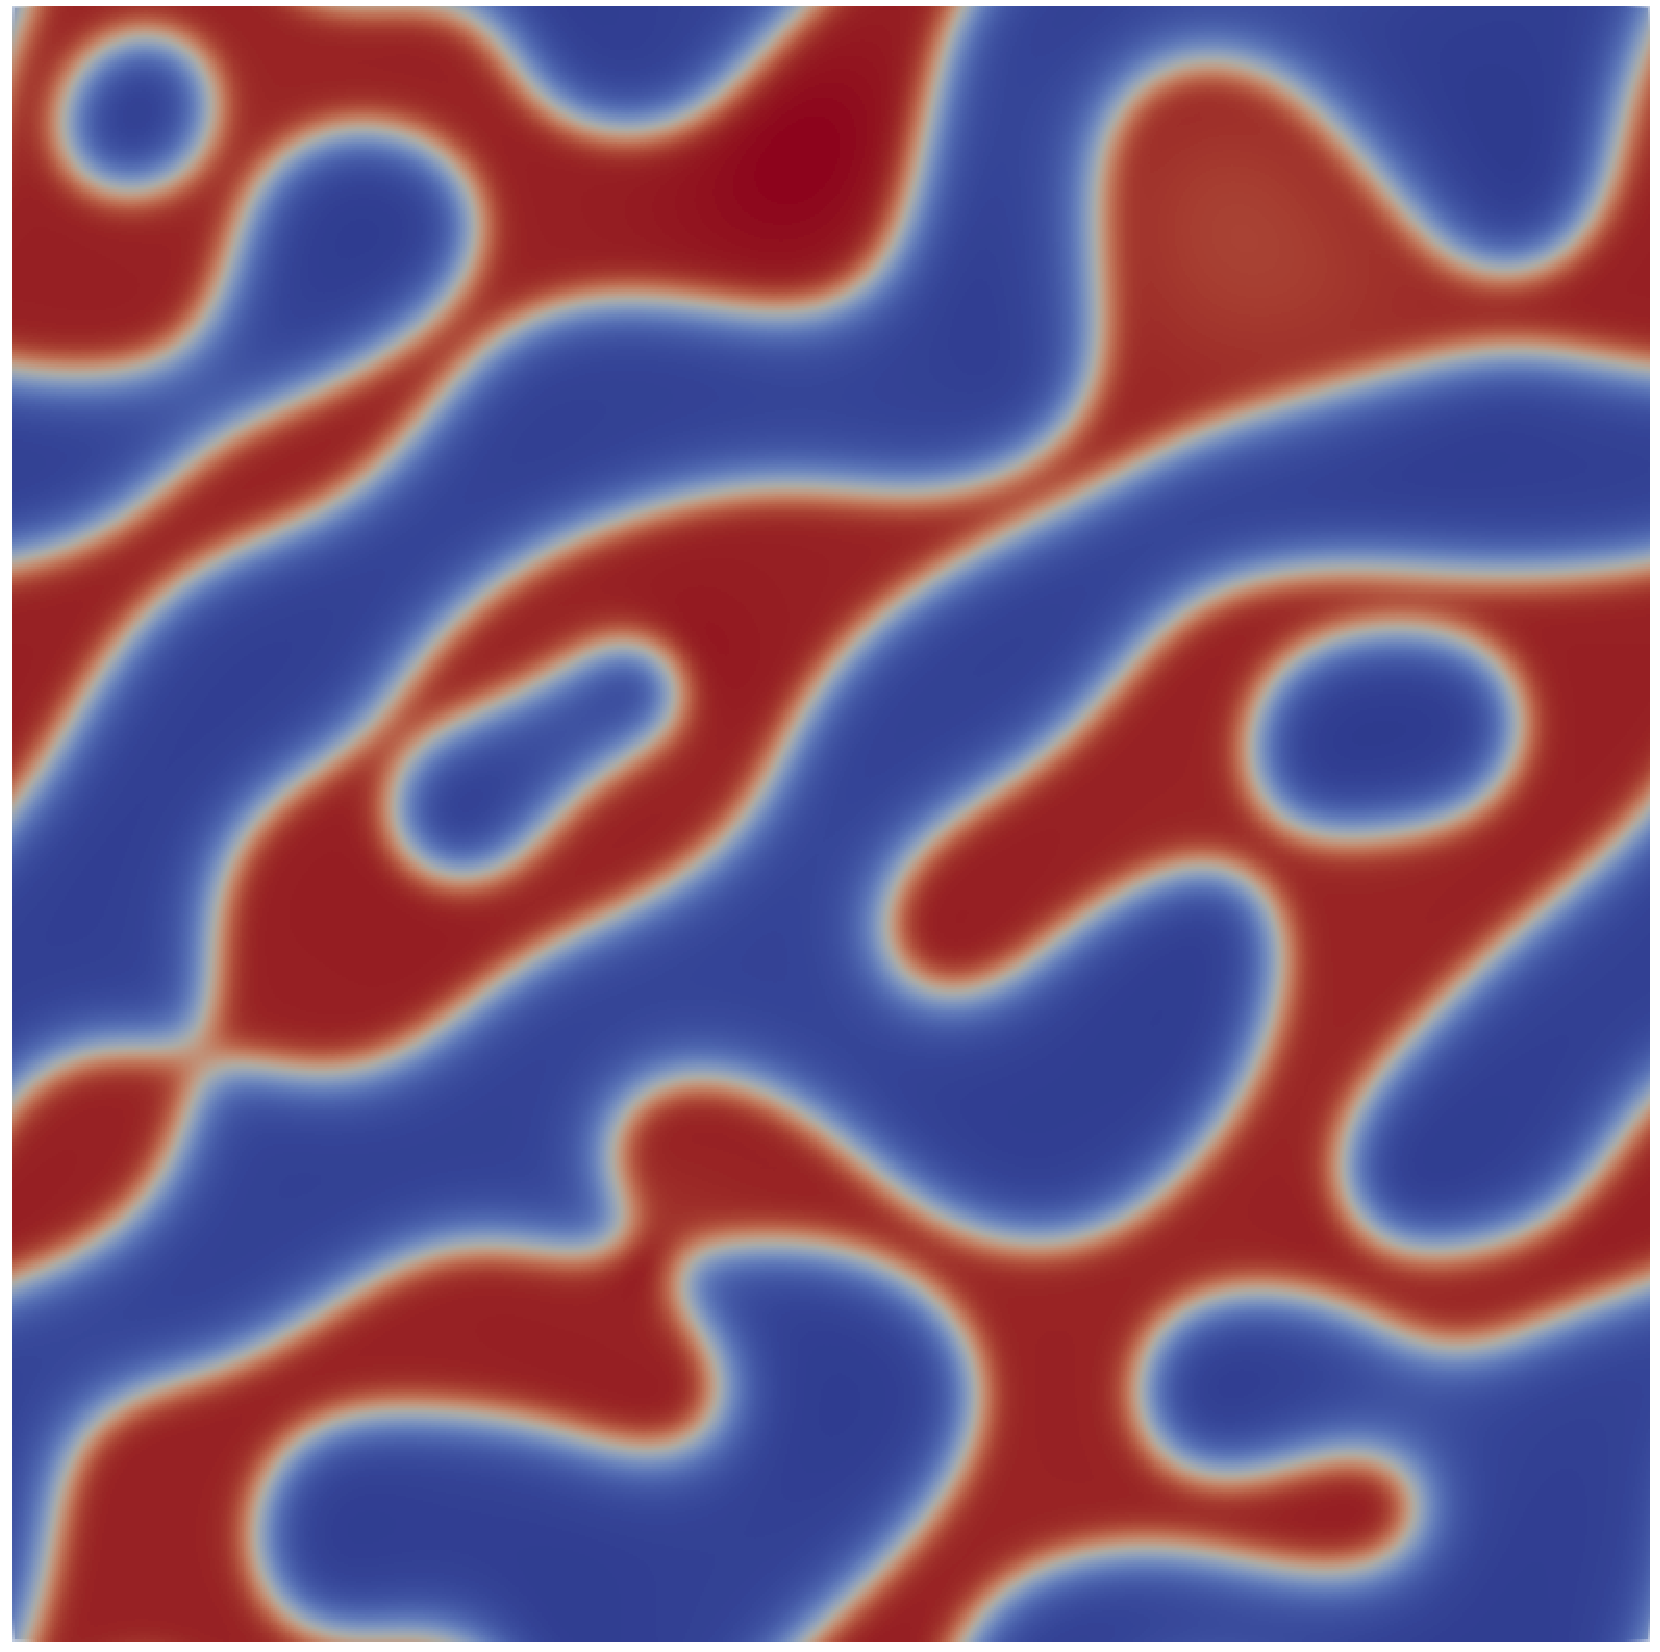
\includegraphics[width=0.95\textwidth]{Imagenes/Maxwell2D/Maxwell2D_sim/Imagenes/t_1000}
        \caption{$t = 1000$}
    \end{subfigure}
    \begin{subfigure}[t]{0.45\textwidth}
        \centering
        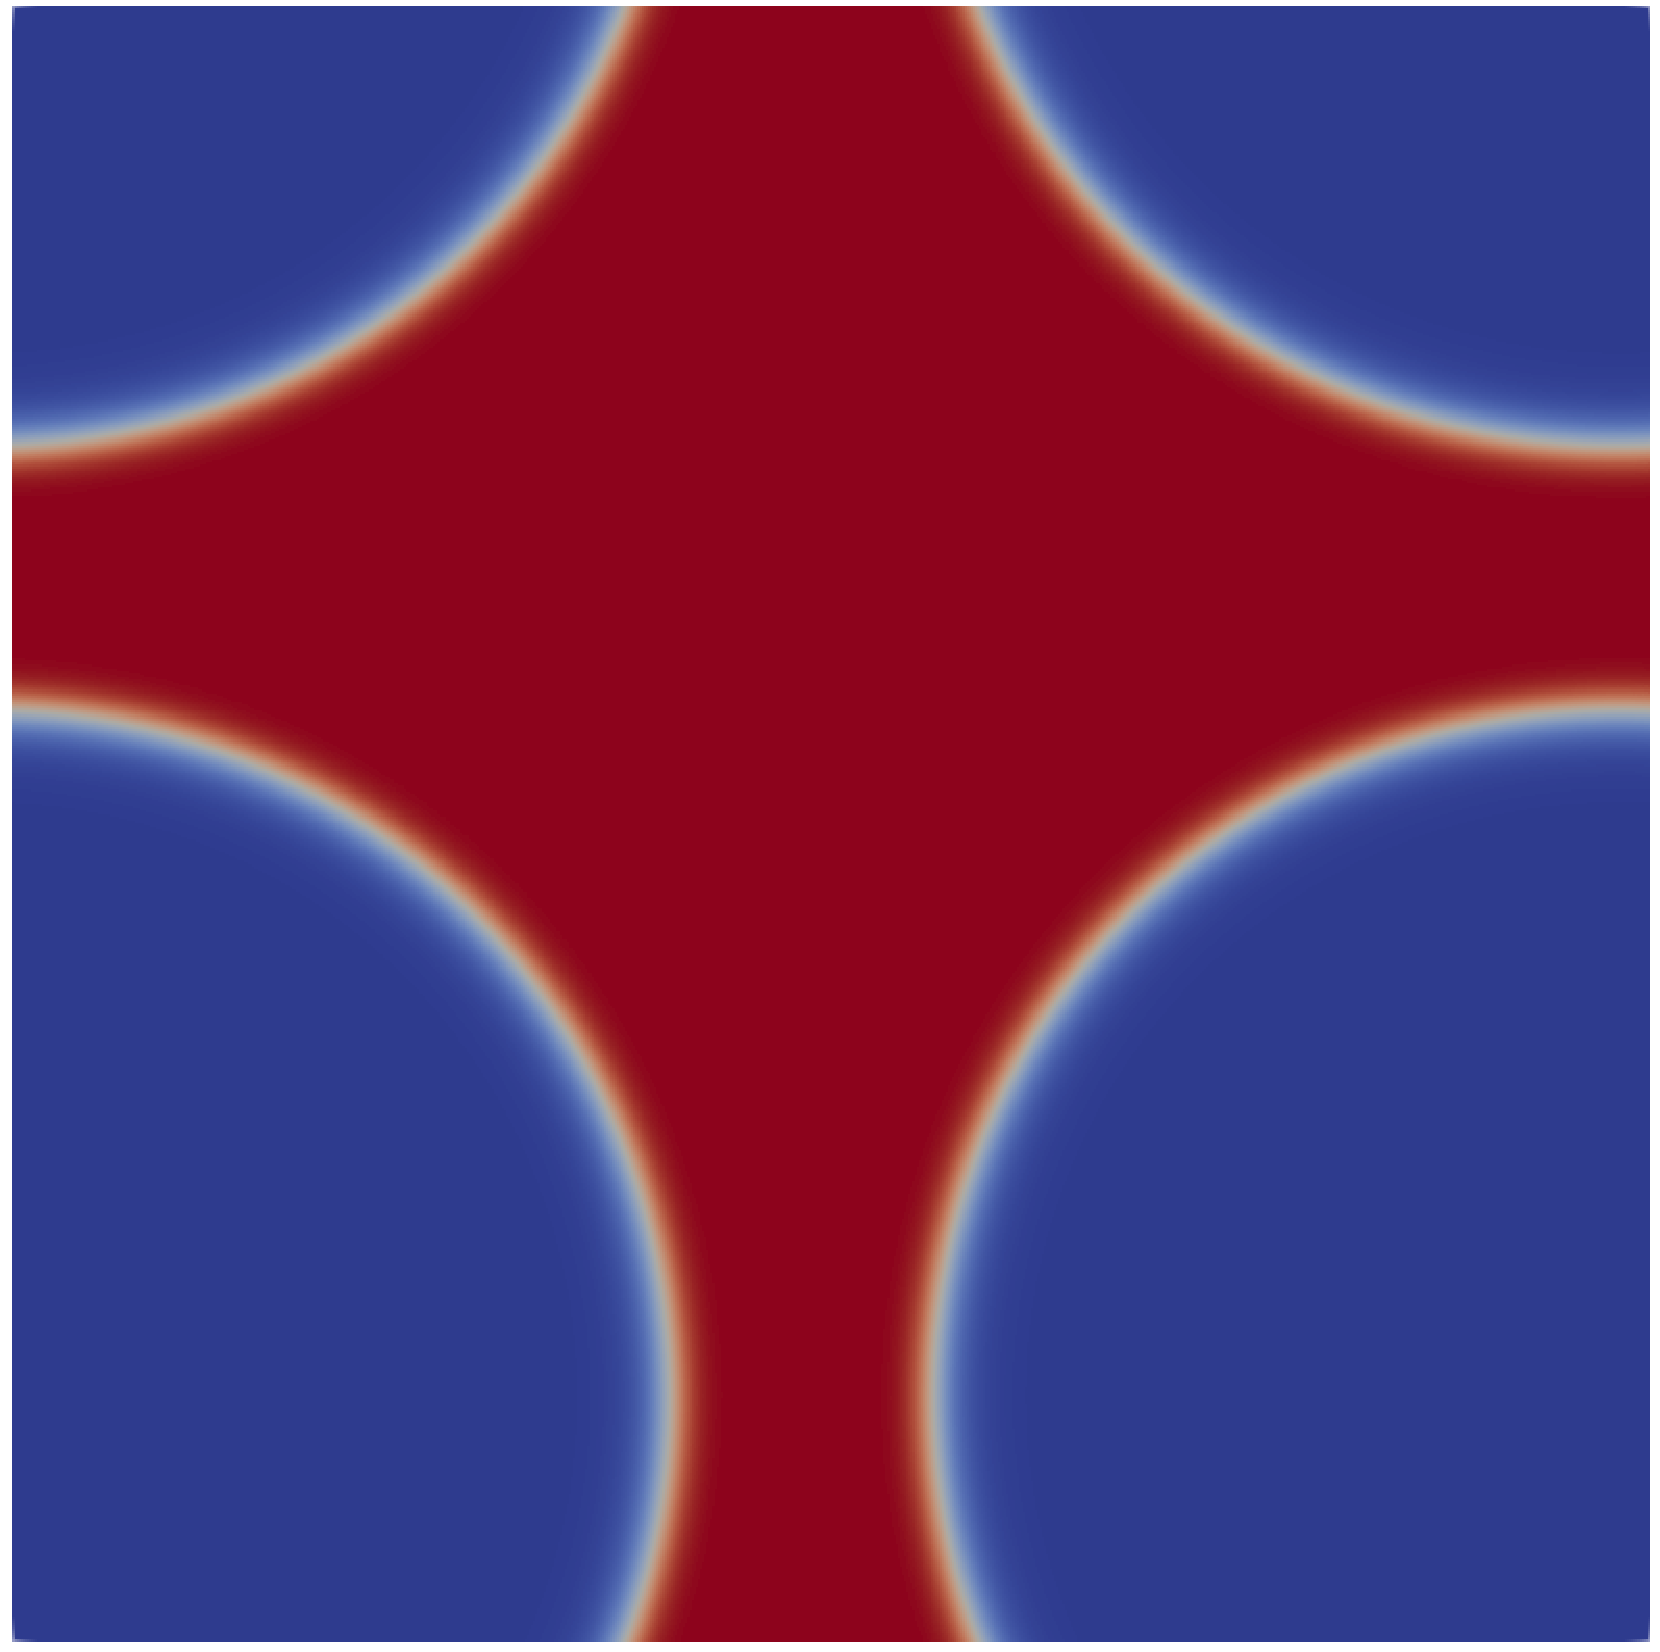
\includegraphics[width=0.95\textwidth]{Imagenes/Maxwell2D/Maxwell2D_sim/Imagenes/t_50000}
        \caption{$t = 50000$}
    \end{subfigure}        
    \caption{Evoluci\'on de una regi\'on bidimensional, peri\'odica, isot\'ermica y sin fuerzas externas, usada para verificar la regla de construcci\'on de Maxwell.}
    \label{fig:maxwell_2d}
\end{figure}
\FloatBarrier

Este problema de ejemplo resulta extremadamente \'util para evaluar el comportamiento del modelo de Li, en particular el efecto de la constante libre $\sigma$ sobre las densidades de coexistencia reproducidas. Para llevar a cabo esta compraraci\'on se simularon dominios peri\'odicos de $200\times 200$ unidades de grilla (u.g.), incorporando la ecuaci\'on de estado de van der Waals con $a=0.5$ y $b=4$. En todos los casos se utilizaron las constantes $M=1$, $G=-1$, $R=1$, y los factores de relajaci\'on fueron fijados en $\tau_{\rho} = \tau_j=1$, $\tau_{e}^{-1}=\tau_{\zeta}^{-1}=\tau_{q}^{-1}=\tau_{\nu}^{-1}=1.1$. En la \fig{fig:maxwell_vdW} se observa que, de manera similar a lo mostrado en el trabajo original de Li \cite{li_lattice_2013} para la ecuaci\'on de Carnahan-Starling, el par\'ametro libre $\sigma$ puede ajustarse para lograr una reproducci\'on satisfactoria de la curva de coexistencia. En este caso, el uso de $\sigma=1/8$ conduce a densidades de coexistencia similares a las obtenidas mediante la regla de Maxwell, para temperaturas reducidas mayores que $0.5$. A partir de la \fig{fig:maxwell_vdW} tambi\'en es posible inferir que con la versi\'on original de un modelo \pp{} MRT, es decir con $\sigma=0$, queda limitado el rango de temperatura en el que se corrige satisfactoriamente la inconsistencia termodin\'amica.
\nomenclature[A]{u.g.}{Unidades de grilla}

\begin{figure}[ht]
	\centering
	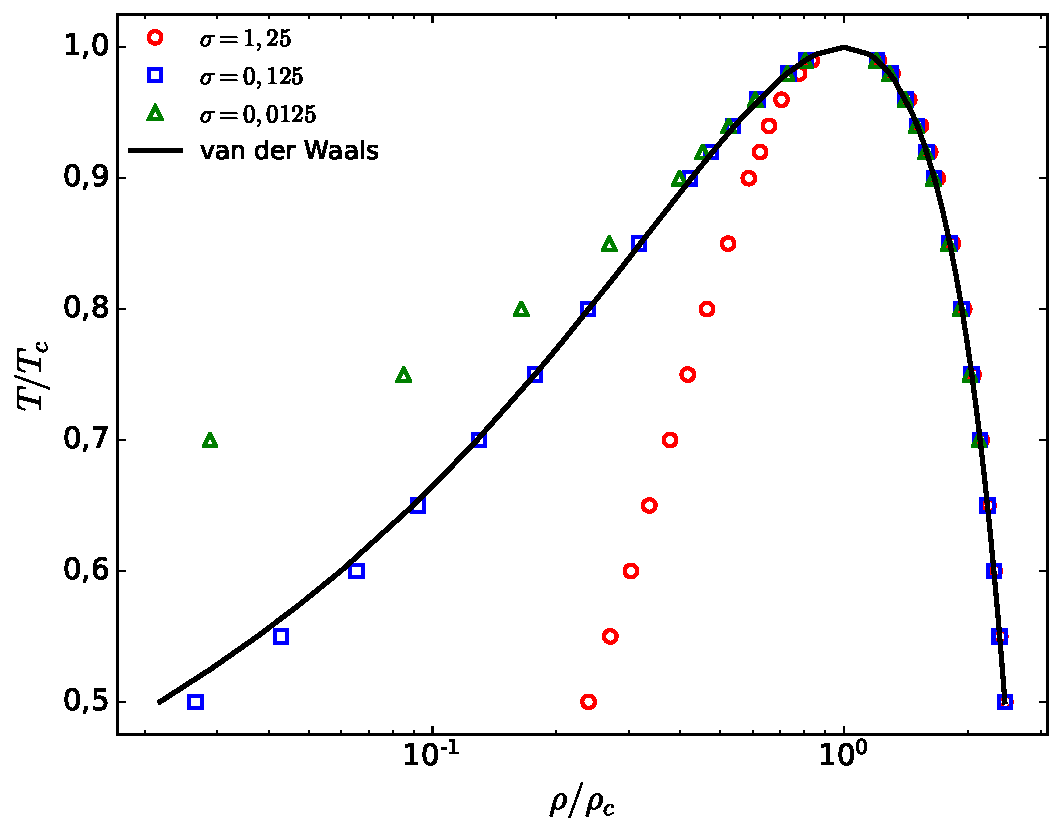
\includegraphics[width=0.75\textwidth]{Maxwell2D/Coexistencia/vdW_sigma}
	\caption{Densidades de coexistencia para la ecuaci\'on de estado de van der Waals, utilizando diferentes valores de $\sigma$. La l\'inea continua corresponde a la regla de construcci\'on de Maxwell.}
	\label{fig:maxwell_vdW}
\end{figure}

Es importante destacar que si se observaron diferencias significativas en la reproducci\'on de la curva de coexistencia para distintos factores de relajaci\'on. Sin embargo, el valor de $\sigma$ m\'as adecuado est\'a vinculado a los valores de las constantes $a$ y $b$, como se muestra en la \fig{fig:maxwell_vdW_eos}, y por lo tanto debe recalcularse para cada EOS y conjunto de par\'ametros libres.

\begin{figure}[ht]
	\centering
	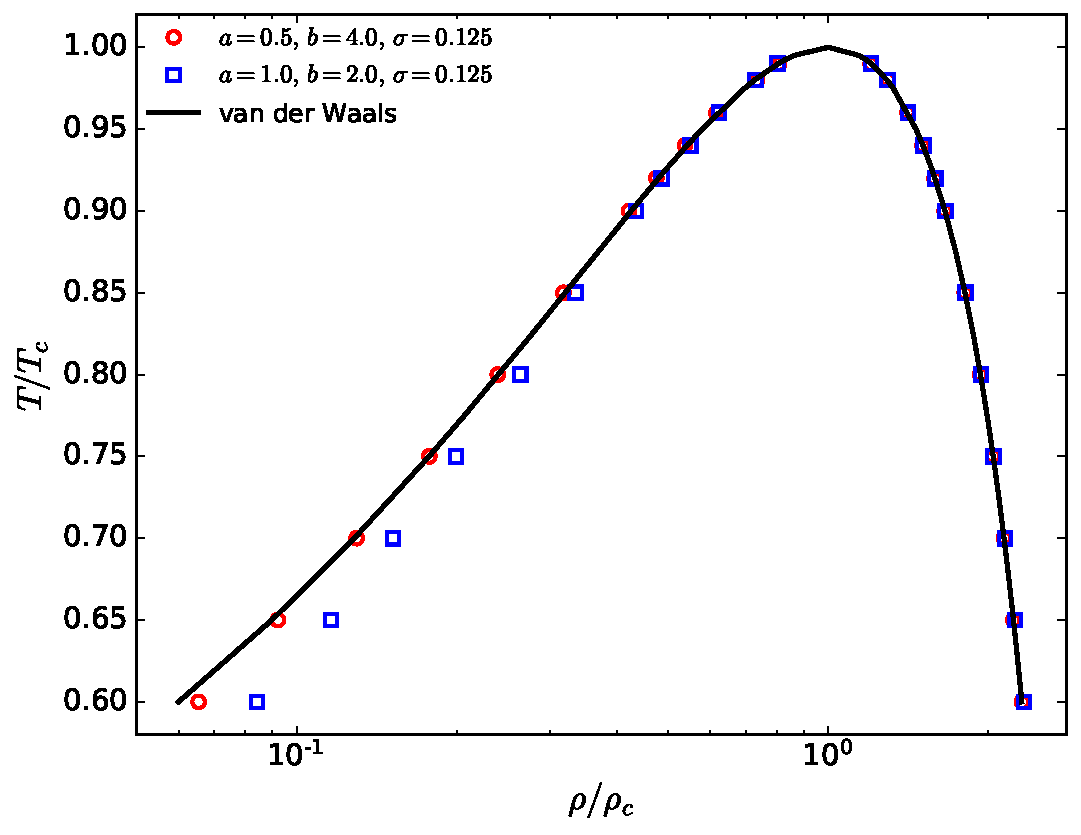
\includegraphics[width=0.75\textwidth]{Maxwell2D/Sigma_eos_const/vdW_sigma_eos}
	\caption{Densidades de coexistencia para la ecuaci\'on de estado de van der Waals, utilizando diferentes constantes para la ecuaci\'on de estado. La l\'inea continua corresponde a la regla de construcci\'on de Maxwell.}
	\label{fig:maxwell_vdW_eos}
\end{figure}


\subsection{Estratificaci\'on de un fluido van der Waals}
\label{sec:vdw_1d}

La validaci\'on de un m\'etodo num\'erico destinado a la resoluci\'on de flujo multif\'asico no es una tarea sencilla, ya que muchas veces no se cuenta con soluciones de referencia que sirvan como base de comparaci\'on. En el caso de LB, tradicionalmente se ha utilizado una gran variedad de problemas como casos de validaci\'on; adem\'as de los ya mencionados, como medici\'on del per\'iodo de oscilaci\'on de droplets o estudio de impacto de droplets sobre superficies planas, es posible adicionar otros como el decaimiento de v\'ortices de Taylor \cite{guo_discrete_2002}, ondas de capilaridad \cite{mccracken_multiple-relaxation-time_2005} o inestabilidades de Rayleigh-Taylor \cite{li_additional_2012}. En estos casos, la figura de m\'erito de la comparaci\'on suele ser una magnitud global de la simulaci\'on, como la velocidad de avance de una interfase, o la amplitud y per\'iodo de una oscilaci\'on inducida. Si bien el seguimiento de estos par\'ametros es v\'alido para establecer una caracterizaci\'on de la precisi\'on del m\'etodo, en este proceso resulta dif\'icil de identificar, en un mismo problema, caracter\'isticas de una simulaci\'on propia de un modelo \pp{}: densidades de coexistencia, ancho de interfase, efecto de fuerzas volum\'etricas o resoluci\'on de grilla.

Esta necesidad de complementar la validaci\'on de un modelo \pp{} llev\'o a la adaptaci\'on y expansi\'on de una soluci\'on anal\'itica originalmente presentada por Berberan-Santos y colaboradores \cite{berberan-santos_liquidvapor_2002}, que permite determinar el perfil de densidad de un fluido ligado a una EOS de vdW, contenido dentro de una cavidad y bajo acci\'on de una fuerza gravitatoria.  Los primeros resultados de este an\'alisis fueron publicados oportunamente en \cite{fogliatto_simulation_2019}.

La idea detr\'as de este problema es conceptualmente sencilla. Si se tiene un fluido dentro de un campo gravitacional uniforme, con gravedad en el sentido negativo de la coordenada $y$, entonces la distribuci\'on est\'atica de presi\'on satisface:
\begin{equation}
	\dfrac{dp}{dy} = -g\rho(y) = -MgC(y),
	\label{eq:p_hidrost}
\end{equation}
donde $M$ corresponde a la masa molar y $C=1/v$ a la concentraci\'on molar. Si la presi\'on del fluido est\'a asociada a la EOS de vdW:
\begin{equation}
	p = \dfrac{RT}{v-b} - \dfrac{a}{v^2} = \dfrac{RT}{1/C-b} - aC^2,
\end{equation}
y se considera que la temperatura puede variar con la coordenada $y$, entonces la \eq{eq:p_hidrost} puede escribirse como
\begin{equation}
	\begin{array}{rcl}
		\dfrac{dp}{dy} &=& \dfrac{\partial p }{\partial C} \dfrac{\partial C}{\partial y}	 + \dfrac{\partial p}{\partial T}\dfrac{\partial T}{\partial y} \\[3mm]
		&=& \dfrac{\partial C}{\partial y}\left[ \dfrac{RT(1/C^2)- 2aC(1/C-b)^2}{(1/C-b)^2} \right] + \dfrac{\partial T}{\partial y}\left( \dfrac{R}{1/C-b}\right)
	\end{array}
	\label{eq:partial_p}
\end{equation}

Combinando las \eqs{eq:p_hidrost}{eq:partial_p} puede obtenerse una ecuaci\'on diferencial para la distribuci\'on de la concentraci\'on molar:
\begin{equation}
	\dfrac{\partial C}{\partial y} = -\left[ MgC + \dfrac{\partial T}{\partial y}\left( \dfrac{RC}{1-bC} \right) \right] \left[ \dfrac{RT}{(1-bC)^2} -2aC \right]^{-1}.
	\label{eq:vdw_molar}
\end{equation} 

La \eq{eq:vdw_molar} corresponde a una ecuaci\'on diferencial ordinaria y no lineal para la concentraci\'on molar, de modo que a trav\'es de su adecuada resoluci\'on es posible calcular la distribuci\'on de densidad dentro de la cavidad. 
La b\'usqueda de esta soluci\'on puede simplificarse si se hace uso de la ley de similaridad mostrada en la Secci\'on~\ref{sec:EOS}. En particular, es necesario introducir las variables adimensionales
\begin{equation}
	E_r = \dfrac{Mgy}{RT_c}, \qquad \rho_r=Cv_c=\dfrac{\rho}{\rho_c}, \qquad p_r=\dfrac{p}{p_c}, \qquad T_r = \dfrac{T}{T_c}, \qquad v_c = 3b,
\end{equation}
donde $E_r$ se denota como energ\'ia gravitacional reducida. De esta forma, si se incorporan las variables adimensionales a la \eq{eq:vdw_molar}, es posible obtener una ecuaci\'on diferencial expresada \'unicamente en unidades reducidas:
\begin{equation}
	\dfrac{d\rho_r}{dE_r} = -\left[ \rho_r + \dfrac{dT_r}{dE_r} \left( \dfrac{\rho_r}{1-\rho_r/3} \right) \right]
\left[ \dfrac{T_r}{(1-\rho_r/3)^2} -\dfrac{9}{4}\rho_r \right]^{-1}.
	\label{eq:vdw_column_red}
\end{equation}
\nomenclature[N]{$E_r$}{Energ\'ia gravitacional reducida}

La integraci\'on de la \eq{eq:vdw_column_red} debe realizarse a partir de la ubicaci\'on de la interfase, $E_r = E_{r_0}$, y requiere como condici\'on inicial a las densidades de coexistencia. De esta forma, la integraci\'on se realiza considerando $\rho_r(E_{r_0}) = \rho_{g_r}$ para $E_r > E_{r_0}$ y $\rho_r(E_{r_0}) = \rho_{l_r}$ para $E_r < E_{r_0}$. En el caso de la EOS de vdW, la integral de la regla de construcci\'on de Maxwell puede resolverse de manera anal\'itica:
\begin{equation}
	\begin{aligned}
	\int_{v_l}^{v_g} p_0 \, \mbox{d}v' &= \int_{v_l}^{v_g} \left( \dfrac{RT}{v'-b} - \dfrac{a}{v'^2} \right) \mbox{d}v' \\
		p_0(v_g-v_l) &= RT \ln \left( \dfrac{v_g - b}{v_l-b} \right) + a\left( \dfrac{1}{v_g} - \dfrac{1}{v_l} \right)
	\end{aligned}
	\label{eq:vdw_maxwell_analitica}
\end{equation}


La \eq{eq:vdw_maxwell_analitica} tambi\'en puede escribirse usando variables reducidas:
\begin{equation}
	8T_r \ln \left( \dfrac{3/\rho_{g_r}-1}{3/\rho_{l_r}-1} \right) + 9(\rho_{g_r} - \rho_{l_r}) = 3p_{0_r} \left( \dfrac{1}{\rho_g} - \dfrac{1}{\rho_l} \right)
\end{equation}
donde $p_{0_r}$ corresponde a la presi\'on de saturaci\'on reducida. Es particular, si se expresa a la ecuaci\'on de estado de van der Waals en unidades reducidas:
\begin{equation}
 p_r = \dfrac{8 T_r}{3/\rho_r-1} - 3\rho_r,
\end{equation}
entonces puede usarse la igualdad $p_r(\rho_{g_r}) = p_r(\rho_{l_r})$ para obtener una relaci\'on entre la temperatura reducida y las densidades de coexistencia:
\begin{equation}
	T_r = \dfrac{1}{8}(\rho_{l_r}+\rho_{g_r})(3-\rho_{l_r})(3-\rho_{g_r})
	\label{eq:tr_maxwell}
\end{equation}

Usando esta expresi\'on de $T_r$ para reescribir a la presi\'on de saturaci\'on como:
\begin{equation}
	p_{r_0} = p_r(\rho_{g_r}) = \rho_{g_r} \rho_{l_r} ( 3 - \rho_{l_r} - \rho_{g_r} ),
\end{equation}
finalmente puede escribirse el resultado de la integral de la regla de construcci\'on de Maxwell en unidades reducidas como:
\begin{equation}
	\left( \dfrac{3/\rho_{g_r}-1}{3/\rho_{l_r}-1} \right) = \dfrac{\rho_{l_r} - \rho_{g_r}}{\rho_{l_r} + \rho_{g_r}}\left( \dfrac{3}{3-\rho_{l_r}} + \dfrac{3}{3-\rho_{g_r}} \right).
	\label{eq:rhor_maxwell}
\end{equation}

De esta manera, las \eqs{eq:tr_maxwell}{eq:rhor_maxwell} constituyen un sistema de ecuaciones no lineal que puede ser utilizado para encontrar las densidades de coexistencia $\rho_{l_r}$ y $\rho_{g_r}$ para una temperatura $T_r$.

La resoluci\'on de la distribuci\'on de densidad dentro de una cavidad debe cerrarse con un mecanismo para calcular la posici\'on de la interfase, el cual puede obtenerse a partir de la conservaci\'on de masa inicial de la cavidad:
\begin{equation}
	\begin{gathered}
		\int_{0}^{h_0} C_l(y') \, \mbox{d}y' + \int_{h_0}^{H} C_g(y') \, \mbox{d}y' = \bar{C}H ,\\[3mm]
		\int_{0}^{E_{r_0}} \rho_{l_r} (E'_r) \, \mbox{d}E'_r + \int_{E_{r_0}}^{E_r(H)} \rho_{g_r}(E'_r) \, \mbox{d}E'_r = \bar{\rho_r}E_{r_m}, \\
	\end{gathered}
	\label{eq:masa_maxwell}
\end{equation}
donde $\bar{C}$ y $\bar{\rho_r}$ denotan a los valores promedio de concentraci\'on molar y densidad reducida respectivamente. En resumen, el conjunto de ecuaciones (\ref{eq:vdw_column_red}), (\ref{eq:tr_maxwell}), (\ref{eq:rhor_maxwell}) y (\ref{eq:masa_maxwell}) permite determinar, de manera num\'erica, c\'omo es la distribuci\'on de densidad para un fluido vdW dentro de una cavidad  bajo acci\'on de la gravedad. En este caso, se asume que ambas fases quedan claramente separadas por una interfase de espesor nulo, y que la temperatura en el interior del fluido sigue una distribuci\'on arbitraria, es decir, independiente de la densidad.  Esta \'ultima hip\'otesis en general no es v\'alida, pero aporta cierto grado de flexibilidad a la soluci\'on anal\'itica, y resulta de gran utilidad para evaluar el desempe\~no de un modelo \pp{}. Tomando en cuenta estas caracter\'isticas, el algoritmo implementado para encontrar la distribuci\'on de densidad queda descripto por los siguientes pasos:

\begin{enumerate}

\item Selecci\'on de una discretizaci\'on inicial $\Delta_0$ para el intervalo $[0.E_r(H)]$.

\item Determinaci\'on de perfiles iniciales para la temperatura y densidad reducida. La distribuci\'on de temperatura elegida no cambia con los pasos siguientes.

\item Elecci\'on de una posici\'on inicial para la interfase, $E_{r_0}^{(0)}$.

\item \label{itm:rhor_tr} C\'alculo de las densidades de coexistencia para $T_r(E_{r_0}^{(0)})$ usando las \eqs{eq:tr_maxwell}{eq:rhor_maxwell}.

\item Integraci\'on de la \eq{eq:rhor_maxwell} hacia ambos lados de la interfase usando esquemas de diferencias finitas adelantadas de segundo orden. Espec\'ificamente, si la interfase se encuentra en la posici\'on $E_{r_0}^{(k)}$, donde el supra\'indice $k$ corresponde al n\'umero de iteraci\'on, entonces es necesario integrar a la \eq{eq:rhor_maxwell} entre $E_{r_0}^{(k)}$ y $E_r(H)$ usando
\begin{equation}
	\rho_r(E_{r_j} + 2\Delta) = -3\rho_r(E_{r_j}) + 4\rho_r(E_{r_j} + \Delta) - 2\Delta \left.\dfrac{d \rho_r}{d E_r} \right|_{E_{r_j}},
\end{equation}
donde se define la posici\'on $E_{r_j} = E_{r_0}^{(k)} + j\Delta$ y $\Delta$ se calcula mediante
\begin{equation}
	\Delta = \dfrac{E_r(H) - E_{r_0}^{(k)}}{\mbox{int} \left( \dfrac{E_r(H) - E_{r_0}^{(k)}}{\Delta_0} \right)}.
\end{equation}

De esta forma, tomando como condici\'on inicial a a $\rho_r(E_{r_0}^{(k)}) = \rho_{g_r}(E_{r_0}^{(k)})$, puede calcularse la densidad de la fase gaseosa en $\mbox{int}[ (E_r(H) - E_{r_0}^{(k)} )/\Delta_0 ]$ puntos. El procedimiento es similar para la fase l\'iquida, es decir, $E_r \in [0,E_{r_0}^{(k)}]$.

\item C\'alculo del exceso (o defecto) de masa usando la \eq{eq:masa_maxwell}. Si la igualdad no se cumple, debe reubicarse a la interfase en una nueva posici\'on $E_{r_0}^{(k+1)} < E_{r_0}^{(k)}$ si existe exceso de masa, o $E_{r_0}^{(k+1)} > E_{r_0}^{(k)}$ si hay defecto de la misma. La determinaci\'on de esta ubicaci\'on se hace mediante la t\'ecnica de bisecci\'on, es decir, conservando las posiciones l\'imites admisibles a cada lado de la interfase (obtenidas de las iteraciones previas), y eligiendo el punto medio entre la posici\'on actual y el l\'imite correspondiente.

\item Repetici\'on a partir del punto \ref{itm:rhor_tr}, calculando las densidades de coexistencia para $T_r(E_{r_0}^{(k+1)})$ e iterando hasta que la posici\'on de la interfase converja con una tolerancia preestablecida.

\end{enumerate}


La distribuci\'on de densidad en una cavidad constituye un excelente caso de prueba para un modelo \pp{} con EOS de vdW, ya que no s\'olo permite verificar la correcta reproducci\'on de la curva de coexistencia, sino que es posible visualizar el efecto de la inclusi\'on de fuerza gravitatoria, temperatura no uniforme y resoluci\'on de grilla. Para representar este problema con LB se defini\'o una cavidad bidimensional de $L=3$ unidades de grilla en la direcci\'on horizontal ($x$) y $H$ unidades de grilla en la direcci\'on vertical ($y$), como se muestra esquem\'aticamente en la \fig{fig:vdWColumn_cavidad}. Por otro lado, se utiliz\'o una condici\'on de contorno per\'odica en la direcci\'on $x$, y el esquema de no deslizamiento de Zou y He en las caras restantes. En todos los casos mostrados en el presente cap\'itulo, la temperatura en las caras superior e inferior se fij\'o en $T_t$ y $T_b$ respectivamente, con una distribuci\'on lineal en el interior de la cavidad. Por otro lado, salvo que se indique expl\'icitamente lo contrario, en todos los casos se utilizaron las constantes detalladas en la \tb{tab:vdW_isot}.


\begin{figure}[ht]
	\centering
	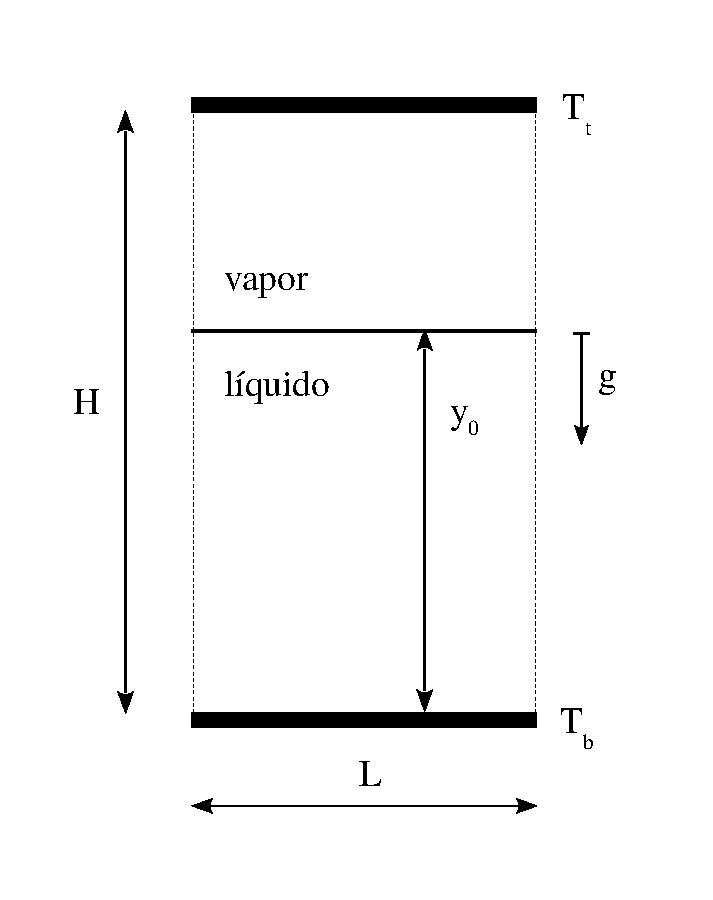
\includegraphics[width=0.6\textwidth]{vdWColumn/cavidad}
	\caption{Esquema del dominio empleado las simulaciones de un fluido van der Waals dentro de una cavidad.}
	\label{fig:vdWColumn_cavidad}
\end{figure}

\begin{table}[ht]
	\centering
    \begin{tabular}{c c}
	    \toprule
        \bf Propiedad & \bf Valor \\
        \midrule
        $\tau_{\rho}^{-1}$, $\tau_{j}^{-1}$ & $1.0$\\
        $\tau_{e}^{-1}$, $\tau_{\zeta}^{-1}$, $\tau_{q}^{-1}$ & $1.1$ \\
        $\tau_{\nu}^{-1}$ & $1.1$ \\
        $\sigma$ & $0.125$ \\
		a & $0.5$ \\
		b & $4$ \\
		M & $1$ \\
		G & $-1$ \\
		R & $1$ \\
        \bottomrule
	\end{tabular}
	\caption{Constantes de simulaci\'on para el problema de estratificaci\'on de un fluido vdW sin transferencia de calor.}
	\label{tab:vdW_isot}
\end{table}  
\FloatBarrier

Siguiendo un procedimiento similar al empleado en los problemas de construcci\'on de Maxwell, las simulaciones de inicializaron con una distribuci\'on de densidad perturbada aleatoriamente en $\pm1\%$ alrededor de un valor elegido, y en este caso se dejaron evolucionar hasta alcanzar un estado estacionario. Por otro lado, el valor de $g$ empleado en el t\'ermino de fuerza volum\'etrica se determin\'o a partir del par\'ametro adimensional $E_r(H)$.

En una primera prueba num\'erica, se utiliz\'o una cavidad con $H=300$, $E_r(H)=10^{-3}$, temperatura uniforme ($T_t = T_b = T_r$) y una densidad inicial (perturbada) igual a la cr\'itica, es decir $\rho_r=1$ . En la \fig{fig:vdWColumn_evolucion} se muestra, a modo de ejemplo, la distribuci\'on de densidad en una cavidad con $T_r=0.99$ para diferentes instantes de tiempo. Como puede observarse, despu\'es del instante inicial se produce una r\'apida separaci\'on de fases en  bandas horizontales. Como es esperable a partir del balance hidrost\'atico, despu\'es de un tiempo de simulaci\'on suficiente, la fase l\'iquida ocupa la parte inferior del dominio, mientras que la densidad es uniforme a lo largo de la coordenada horizontal.

\begin{figure}[htb]
    \centering
    \begin{subfigure}[t]{0.18\textwidth}
        \centering
        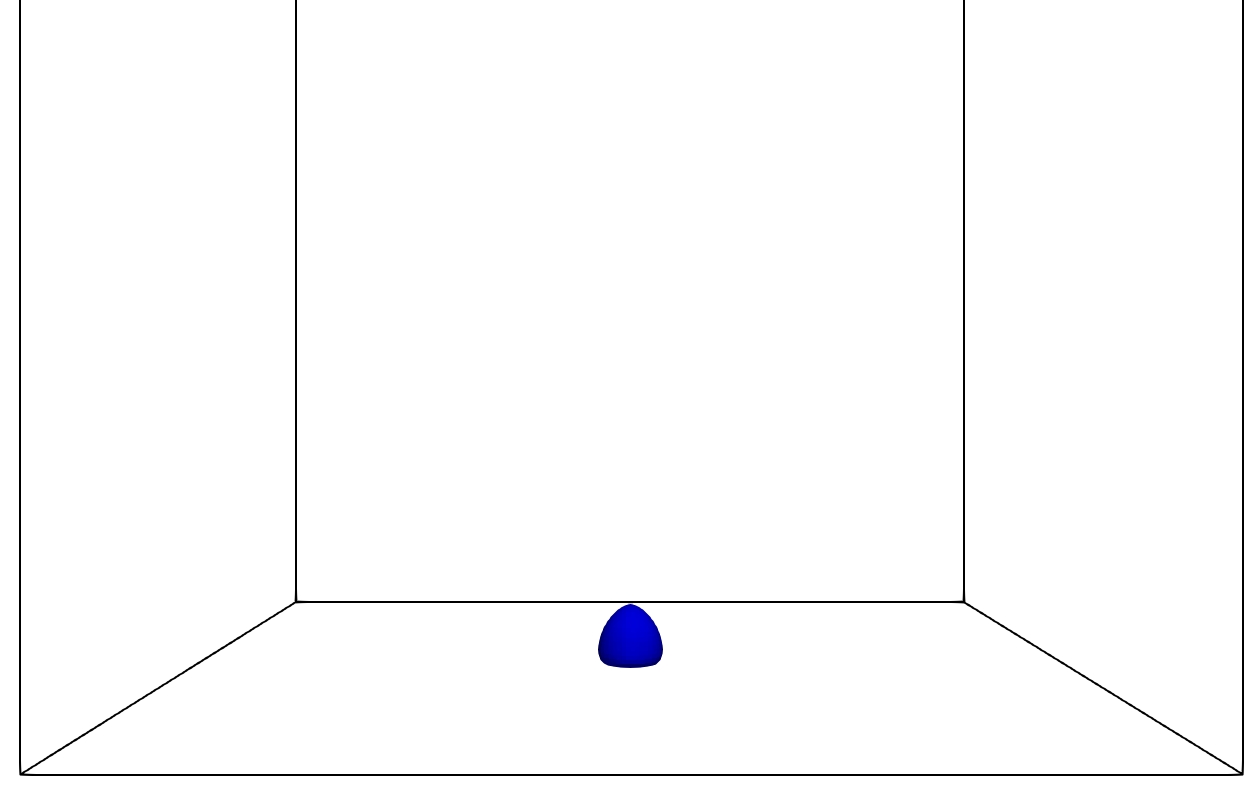
\includegraphics[width=0.95\textwidth]{vdWColumn/Vis/t_0}   
        \caption{$t=0$}     
    \end{subfigure}
    \begin{subfigure}[t]{0.18\textwidth}
        \centering
        \includegraphics[width=0.95\textwidth]{vdWColumn/Vis/t_500}   
        \caption{$t=500$}     
    \end{subfigure}
    \begin{subfigure}[t]{0.18\textwidth}
        \centering
        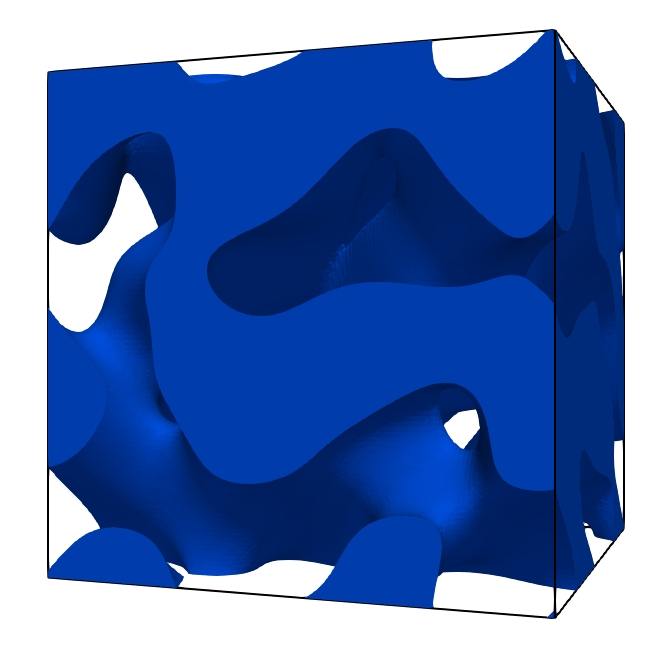
\includegraphics[width=0.95\textwidth]{vdWColumn/Vis/t_1000}   
        \caption{$t=1000$}     
    \end{subfigure}    
    \begin{subfigure}[t]{0.18\textwidth}
        \centering
        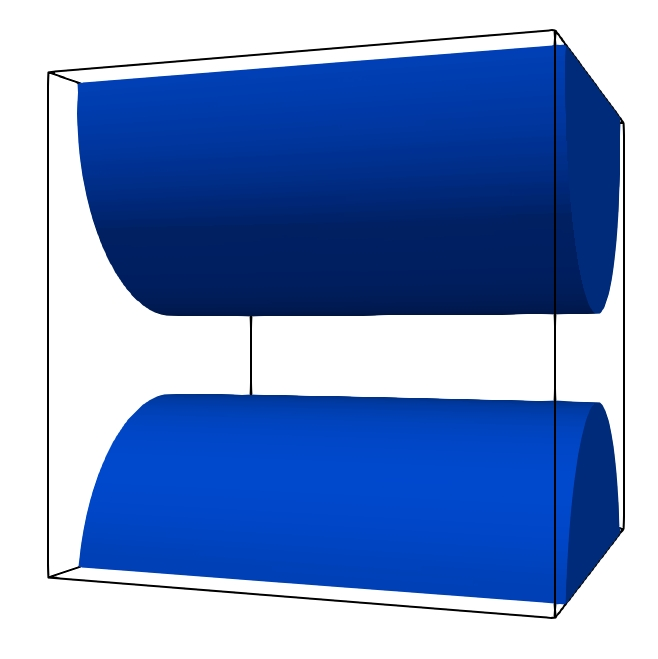
\includegraphics[width=0.95\textwidth]{vdWColumn/Vis/t_10000}   
        \caption{$t=10000$}     
    \end{subfigure}      
    \begin{subfigure}[t]{0.18\textwidth}
        \centering
        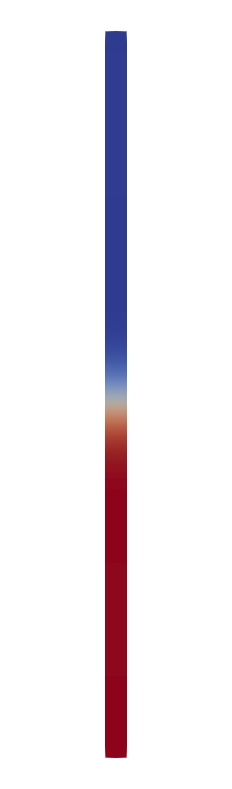
\includegraphics[width=0.95\textwidth]{vdWColumn/Vis/t_50000}   
        \caption{$t=50000$}
    \end{subfigure}      
    \caption{Ejemplo de evoluci\'on de la distribuci\'on de densidad en una columna de fluido van der Waals con temperatura uniforme.}
	\label{fig:vdWColumn_evolucion}
\end{figure}

En la \fig{fig:vdWColumn_rhor_tuniform} se muestran los perfiles de densidad reducida sobre la coordenada vertical, expresada en unidades adimensionales como $y/H = E_r/E_r(H)$. Los perfiles corresponden al resultado de simulaciones con LB para diferentes temperaturas, y se muestran junto con los calculados usando la expresi\'on anal\'itica. Como puede observarse, el modelo \pp{} de Li con $\sigma=0.125$ es capaz de reproducir satisfactoriamente el perfil de densidad en el seno de cada fase, de modo que no se observan efectos apreciables de la fuerza volum\'etrica en la capacidad de correcci\'on de la inconsistencia termodin\'amica. Por otro lado, se observa que el modelo genera una variaci\'on de densidad continua a trav\'es de la interfase, y como se mantienen todas las constantes de simulaci\'on salvo la temperatura del dominio, el espesor de esta interfase disminuye con la temperatura de la cavidad.

\begin{figure}[ht]
	\centering
	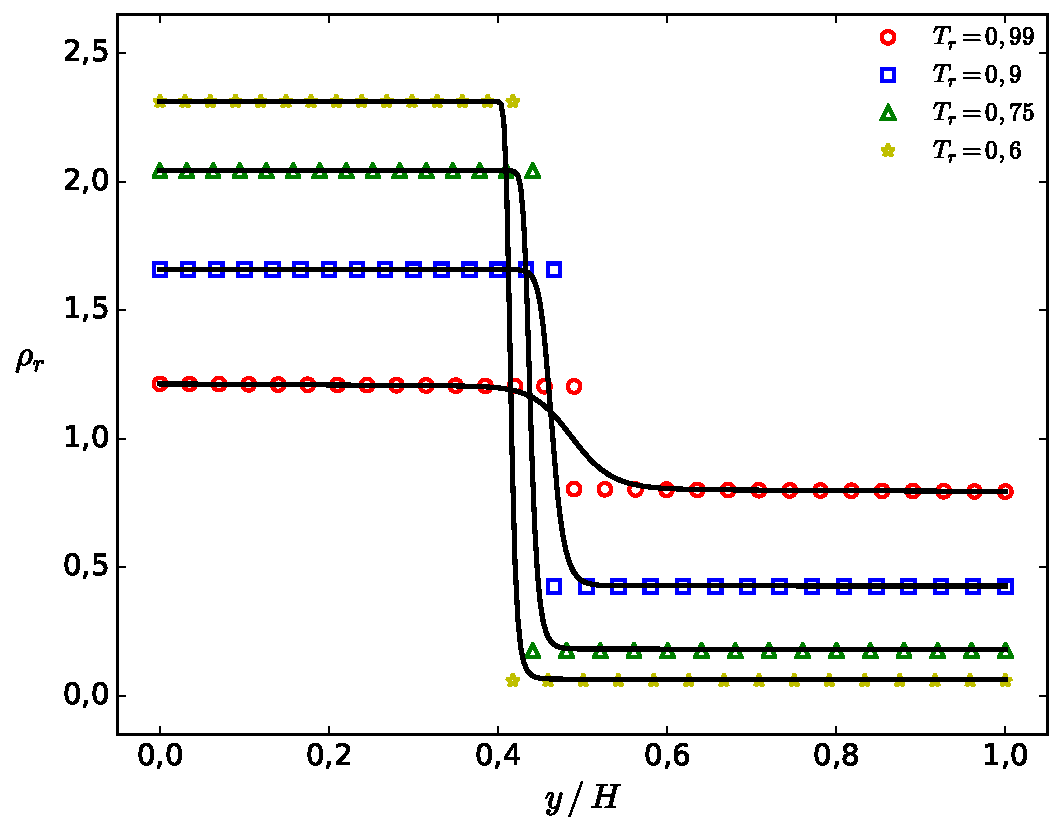
\includegraphics[width=0.75\textwidth]{vdWColumn/TUniform/rhor_vdWcolumn_Tuniform}
	\caption{Distribuci\'on espacial de densidad en una cavidad con fuerza gravitacional dada por $E_r(H)=10^{-3}$. Las l\'ineas continuas corresponden a simulaciones de LB con $\sigma=0.125$, mientras que los puntos representan los valores obtenidos con la expresi\'on anal\'itica.}
	\label{fig:vdWColumn_rhor_tuniform}
\end{figure}

El an\'alisis de la distribuci\'on de densidad puede extenderse al uso de diferentes condiciones iniciales, como la incorporaci\'on de un fluido con distinta densidad promedio. En la \fig{fig:vdWColumn_frac_volumen} se muestra la dependencia de la posici\'on de la interfase (equivalente a fracci\'on de l\'iquido) con la temperatura de la cavidad. En el caso en que la densidad promedio sea igual a la cr\'itica ($\rho_r=1$), las fracciones de l\'iquido y vapor tienden a igualarse a medida que la temperatura se acerca a su valor cr\'itico. Si la densidad promedio es supercr\'itica ($\rho_r > 1$), el volumen de vapor tiende a cero a medida que la temperatura de la cavidad crece, de modo que se observa una temperatura l\'imite a partir de la cual se observa s\'olo una fase l\'iquida. Por otro lado, este comportamiento se invierte para una densidad inicial subcr\'itica ($\rho_r < 1$), por lo que la fracci\'on de fase l\'iquida tiende a cero con el incremento de temperatura. Como se observa en la \fig{fig:vdWColumn_frac_volumen}, este comportamiento predicho por la soluci\'on anal\'itica es reproducido correctamente por el modelo \pp{}.

\begin{figure}[ht]
	\centering
	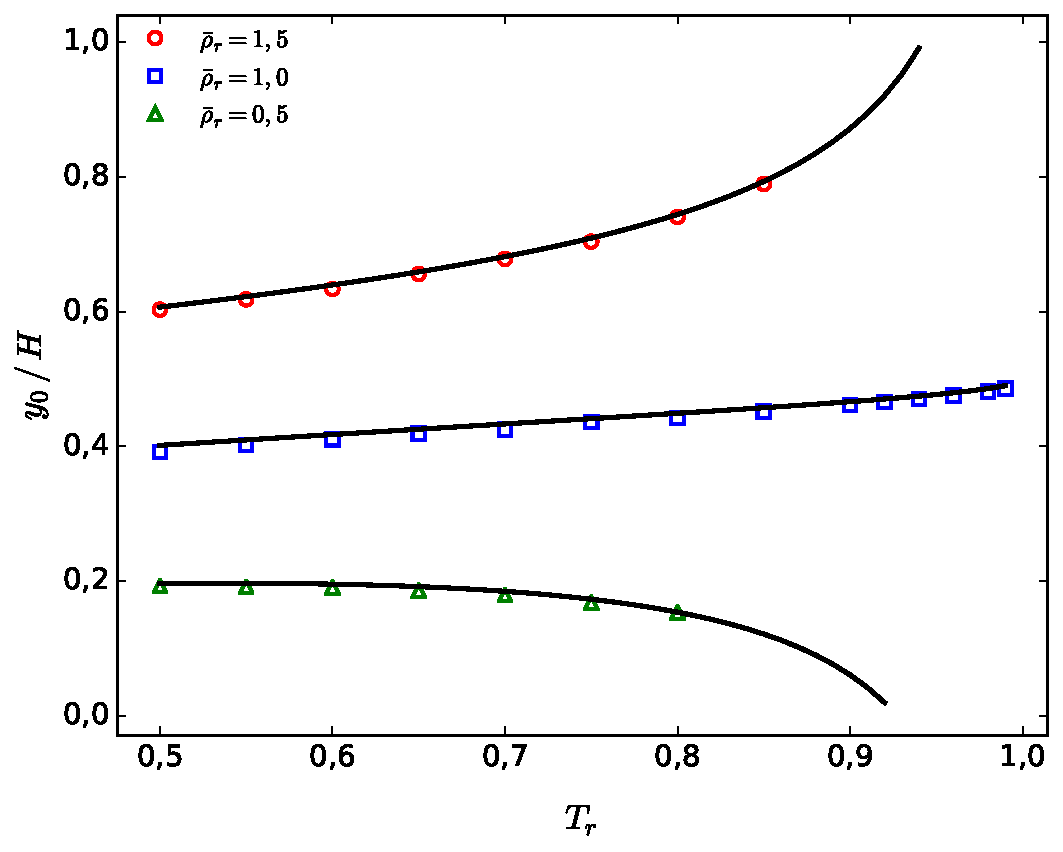
\includegraphics[width=0.75\textwidth]{vdWColumn/frac_volumen/frac_volumen}
	\caption{Posici\'on de la interfase  para diferentes temperaturas en una cavidad con $E_r(H)=10^{-3}$, empleando distintos valores de densidad inicial. Las l\'ineas continuas corresponden a la soluci\'on anal\'itica, mientras que los puntos representan  los resultados de la simulaci\'on con lattice Boltzmann.}
	\label{fig:vdWColumn_frac_volumen}
\end{figure}

Como se mencion\'o anteriormente, uno de los objetivos principales de la comparaci\'on con la soluci\'on anal\'itica consiste en cuantificar los efectos de la fuerza volum\'etrica en la inconsistencia termodin\'amica. Esta influencia puede analizarse a partir de la \fig{fig:vdWColumn_rhor_egrav}, donde se muestran los perfiles de densidad calculados para una cavidad con $T_r=0.99$ y diferentes valores de energ\'ia gravitacional m\'axima. En este caso, los cambios de $E_r(H)$ se reflejaron en las simulaciones a trav\'es de distintos valores de $g$, y los perfiles resultantes se muestran sobre una coordenada normalizada que refleja la distancia a la interfase, es decir, $(y-y_0)/H = (E_r-E_r(y_0)) / E_r(H)$. Como puede apreciarse en la \fig{fig:vdWColumn_rhor_egrav}, el uso de $\sigma=0.125$ permite obtener una representaci\'on adecuada de la distribuci\'on de densidad en el seno del fluido, incluso para valores de $E_r(H)$ elevados.

\begin{figure}[ht]
	\centering
	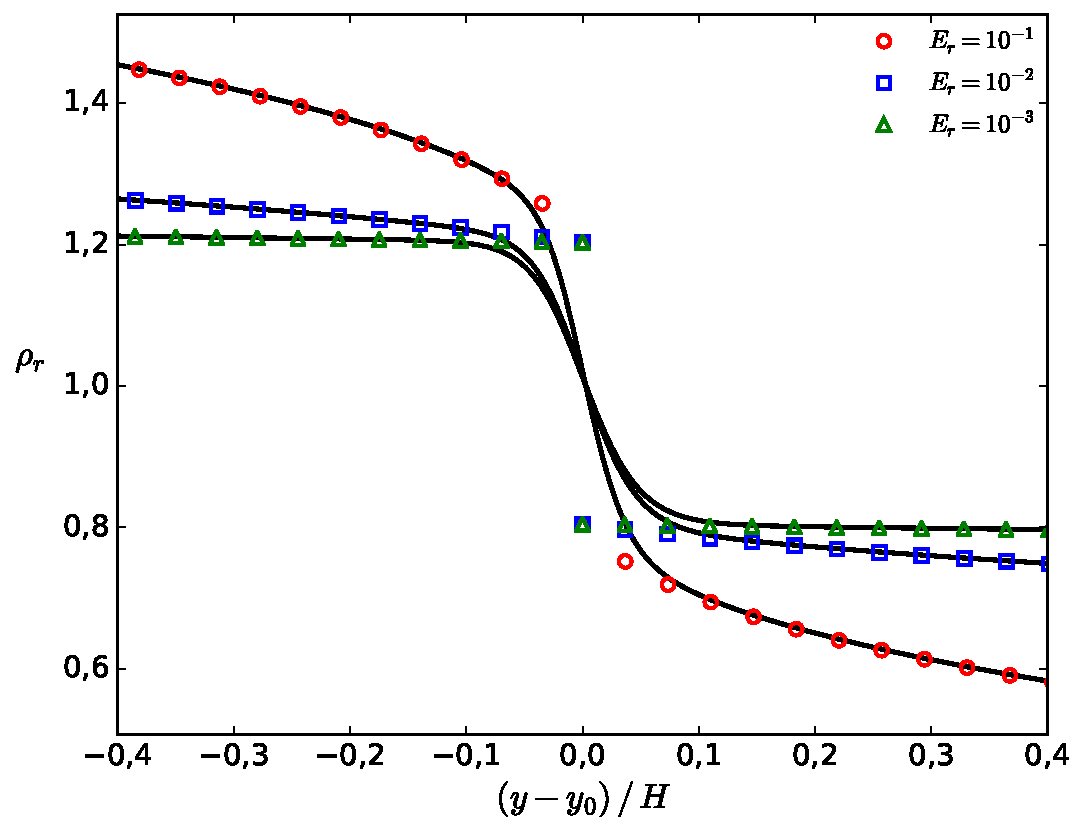
\includegraphics[width=0.75\textwidth]{vdWColumn/energia_grav/rhor_energia_grav}
	\caption{Perfiles de densidad para una cavidad con $T_r = 0.99$ y diferentes $E_r(H)$. Las l\'ineas s\'olidas corresponden a los resultados num\'ericos.}
	\label{fig:vdWColumn_rhor_egrav}
\end{figure}

En los perfiles de densidad mostrados en las \figs{fig:vdWColumn_rhor_tuniform}{fig:vdWColumn_rhor_egrav} se evidencia que, para la misma cantidad de unidades de grilla en la direcci\'on vertical ($H$) e iguales constantes de vdW, la resoluci\'on de la interfase recuperada empeora con el incremento de la temperatura. Por lo tanto, en este punto resulta v\'alido cuestionarse c\'omo es posible mejorar la precisi\'on de la simulaci\'on, que en este caso implica reducir el espesor de la interfase, ya que en el interior de cada fase la representaci\'on es adecuada para las grillas utilizadas.

La primera alternativa consiste en mantener la representaci\'on en unidades reducidas e incrementar $H$. De este modo, se mantienen sin cambios el resto de las contantes de la simulaci\'on a excepci\'on de $g$, que debe adaptarse para conservar el valor de energ\'ia gravitacional reducida m\'axima, $E_r(H) = 10^{-3}$. En la \fig{fig:vdWColumn_rhor_grilla} se observa que la representaci\'on del perfil de densidad reducida, sobre coordenadas adimensionales, produce una mejora consistente en la resoluci\'on de la interfase.

\begin{figure}[ht]
	\centering
	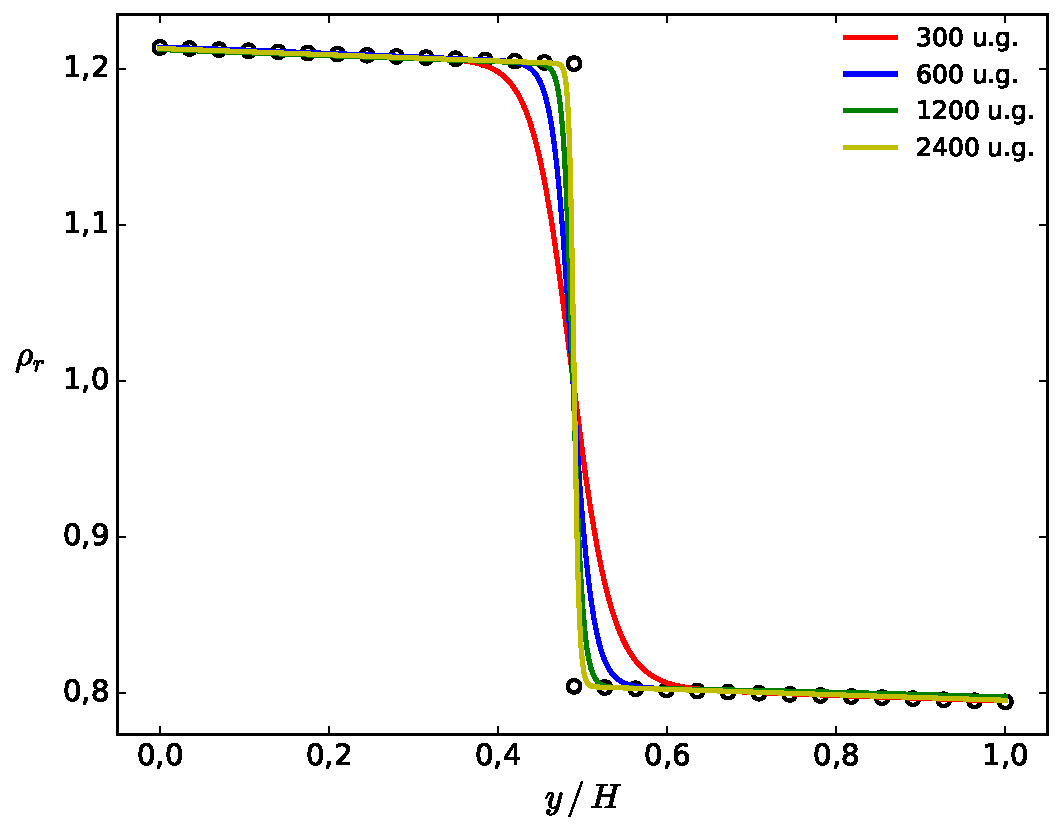
\includegraphics[width=0.75\textwidth]{vdWColumn/TUniform_grilla/rhor_Tuniform_grilla}
	\caption{Perfiles de densidad para una cavidad con $T_r = 0.99$, $E_r(H) = 10^{-3}$ y diferente cantidad de unidades de grilla en la direcci\'on vertical. Los puntos corresponden a la soluci\'on anal\'itica.}
	\label{fig:vdWColumn_rhor_grilla}
\end{figure}
\FloatBarrier

Esta mejora significativa en la reproducci\'on de la interfase se debe, en parte, a que el espesor de la misma se mantiene constante en unidades de grilla, ya que depende exclusivamente de la temperatura reducida y las constantes de la ecuaci\'on de estado. Por lo tanto, es razonabe esperar que, para una misma $T_r$, $E_r(H)$ y $H$, el ancho de la interfase pueda reducirse usando diferentes valores para $a$ y $b$. Este efecto puede apreciarse en las \figs{fig:vdWColumn_b_eos}{fig:vdWColumn_a_eos}, donde se muestran los perfiles de densidad para una cavidad con $T_r=0.99$, $H=300$ y $E_r(H)=10^{-3}$, obtenidos con valores de $b$ fijos ($b=4$) y variando $a$, y viceversa ($a=0.5$). En ambos casos, ya sea incrementando $a$ o disminuyendo $b$, se produce una reducci\'on del espesor de la interfase en unidades de grilla mientras que se conservan los perfiles reducidos en el interior de cada fase. En particular, el incremento del par\'ametro $b$ produce un aumento en la diferencia de densidad absoluta entre cada fase. Por otro lado, el incremento de $a$ y la disminuci\'on de $b$ contribuyen a incrementar el gradiente (dimensional) del potencial de interacci\'on. Ambos efectos contribuyen a mejorar la capacidad del modelo \pp{} para reproducir la interfase, y de esta forma producir una tendencia similar a la observada frente a un incremento en la resoluci\'on de grilla. Sin embargo, es necesario destacar que en este camino se observaron limitaciones de aplicabilidad relacionadas con la estabilidad de la simulaci\'on.

\begin{figure}[ht]
	\centering
	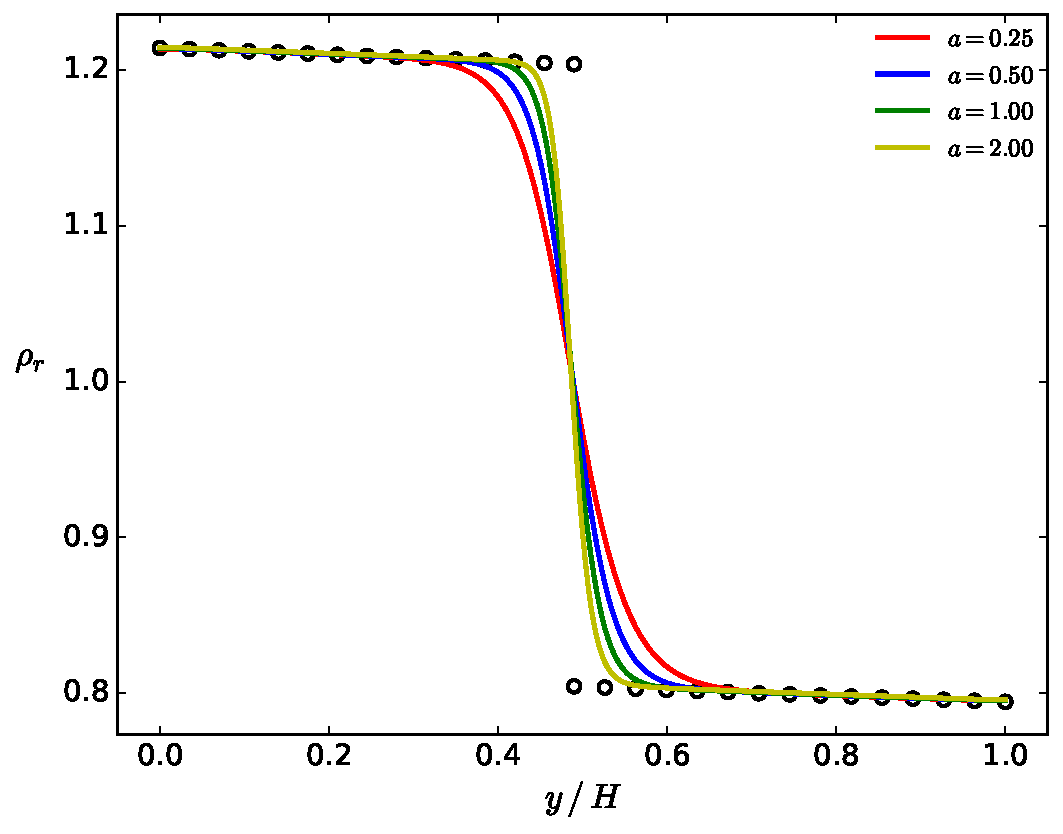
\includegraphics[width=0.75\textwidth]{vdWColumn/TUniform_a_eos/rhor_Tuniform_a_eos}
	\caption{Distribuci\'on espacial de densidad en una cavidad con $T_r = 0.99$. Las l\'ineas continuas corresponden a simulaciones LB con $b=4$ y distintos valores de $a$.}
	\label{fig:vdWColumn_a_eos}
\end{figure}

\begin{figure}[ht]
	\centering
	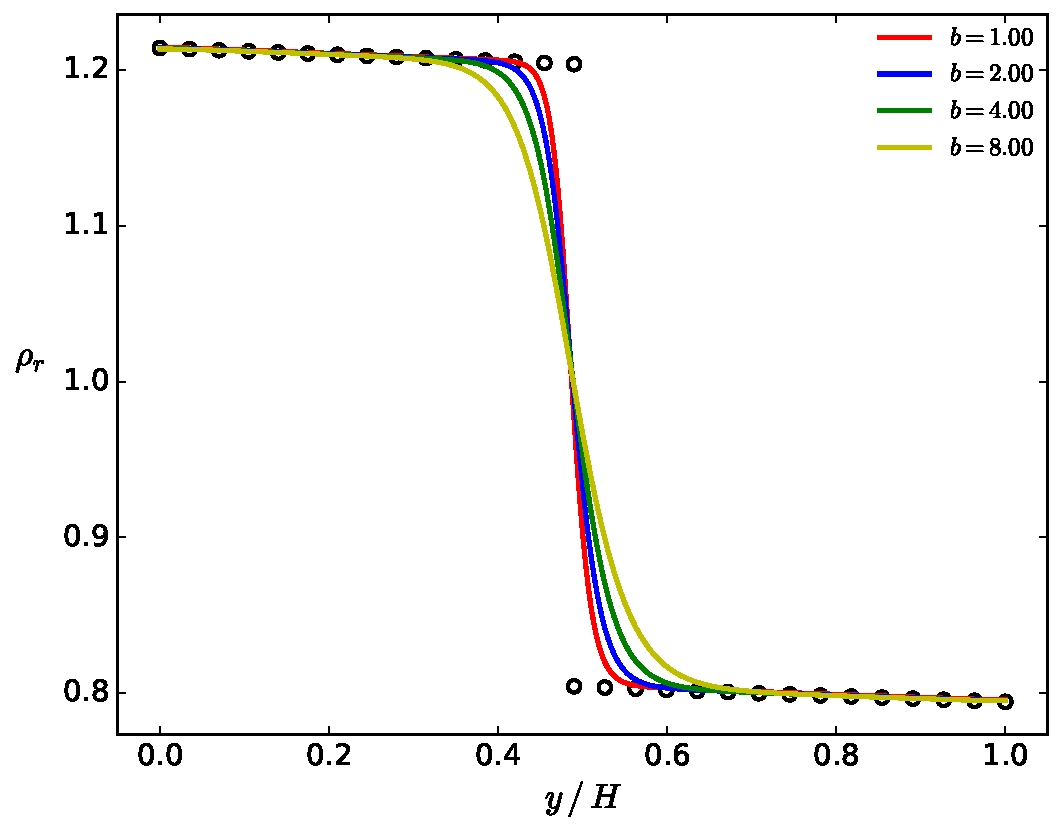
\includegraphics[width=0.75\textwidth]{vdWColumn/TUniform_b_eos/rhor_Tuniform_b_eos}
	\caption{Distribuci\'on espacial de densidad en una cavidad con $T_r = 0.99$. Las l\'ineas continuas corresponden a simulaciones LB con $a=0.5$ y distintos valores de $b$.}
	\label{fig:vdWColumn_b_eos}
\end{figure}
\FloatBarrier

La soluci\'on anal\'itica tambi\'en permite obtener perfiles de densidad en casos donde la distribuci\'on de temperatura no es uniforme. En una segunda prueba num\'erica se utiliz\'o $T_t=0.99$ y se consider\'o una distribuci\'on lineal de temperatura en la cavidad, variando param\'etricamente la temperatura de la cara inferior, $T_b$. El resto de las constantes y propiedades de simulaci\'on permanecen iguales a los casos anteriores.

En la \fig{fig:vdWColumn_rhor_TNonUniform} se muestran los perfiles de densidad obtenidos para diferentes $T_b$. Nuevamente, puede observarse que el modelo \pp{} es capaz de reproducir correctamente la distribuci\'on de densidad en el interior de cada fase, y genera una interfase cuyo espesor disminuye junto con la temperatura de la cara inferior.

\begin{figure}[ht]
	\centering
	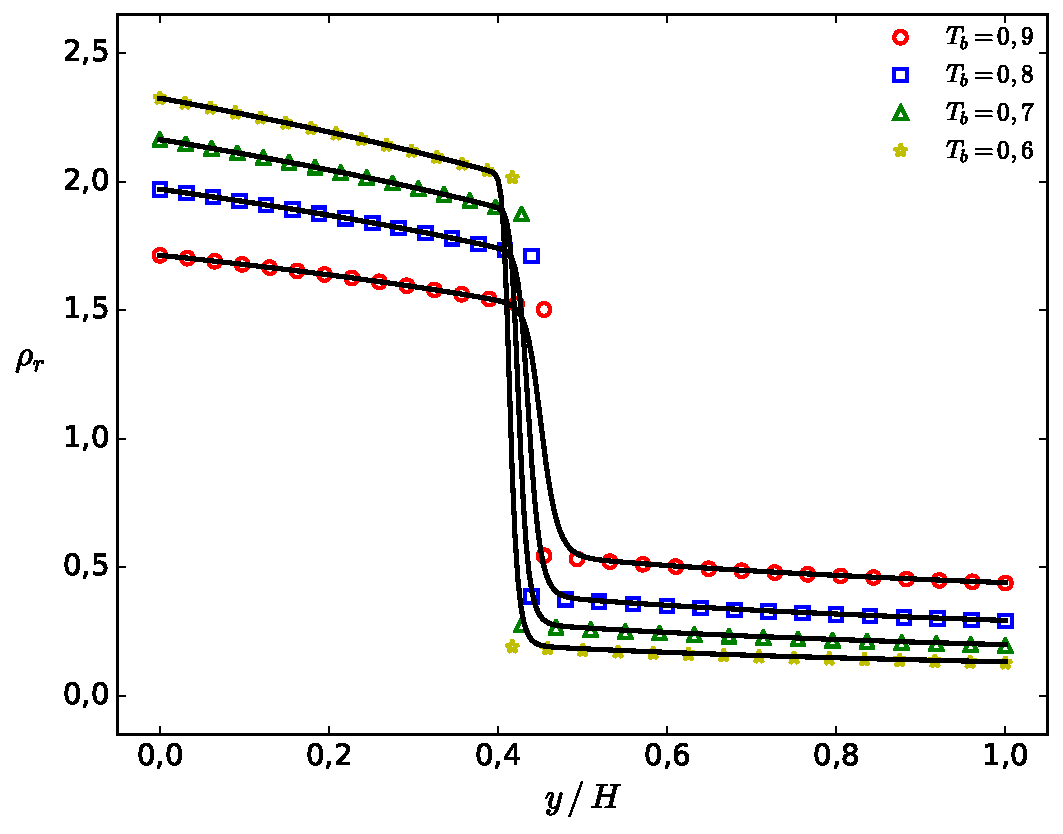
\includegraphics[width=0.75\textwidth]{vdWColumn/TNonUniform/rhor_vdWcolumn_TNonUniform}
	\caption{Perfiles de densidad para una cavidad con $T_t = 0.99$ y una distribuci\'on lineal de temperatura, fijada para diferentes valores de $T_b$. Los puntos corresponden a la soluci\'on anal\'itica.}
	\label{fig:vdWColumn_rhor_TNonUniform}
\end{figure}

Siguiendo la idea de la prueba num\'erica anterior, tambi\'en es posible verificar la consistencia de este m\'etodo \pp{} usando diferentes unidades de grilla en la direcci\'on vertical. Como puede apreciarse en la \fig{fig:vdWColumn_TNonUniform_grilla}, si se incrementa $H$ a la vez que se conservan los dem\'as par\'ametros adimensionales representativos, es posible lograr una reducci\'on consistente y precisa del espesor de la interfase sobre coordenadas adimensionales.

\begin{figure}[ht]
	\centering
	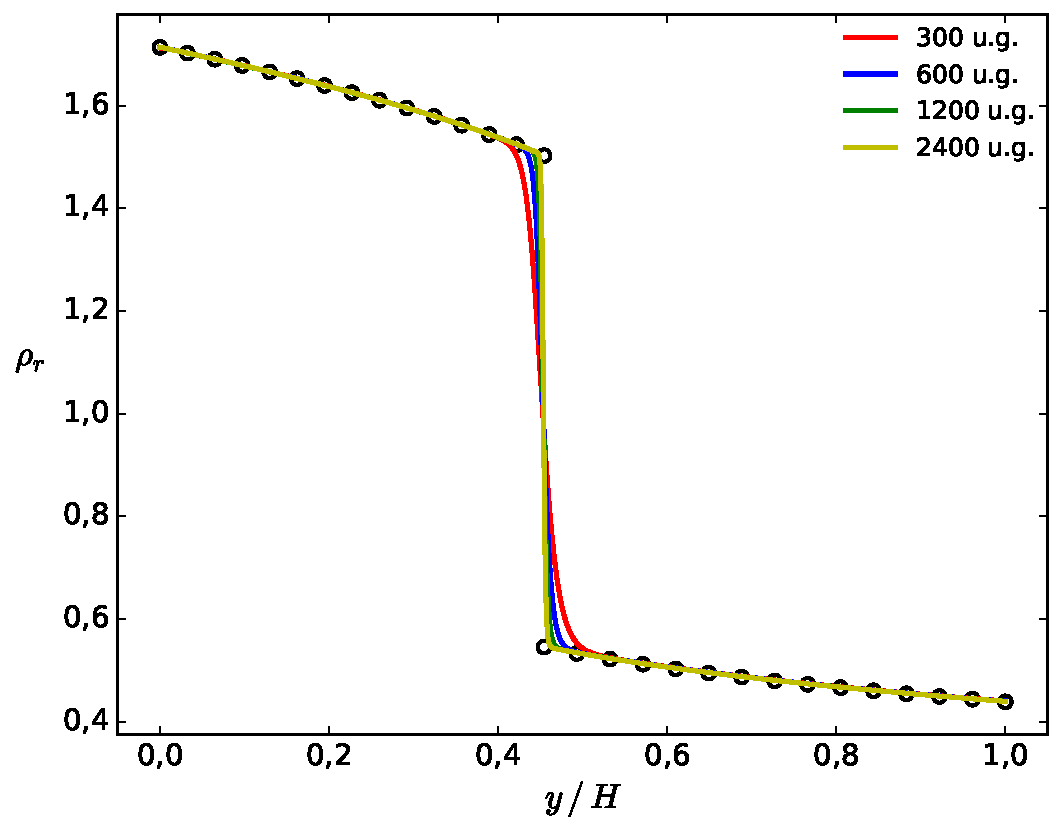
\includegraphics[width=0.75\textwidth]{vdWColumn/TNonUniform_grilla/rhor_TNonUniform_grilla}
	\caption{Perfiles de densidad para una cavidad con $T_t = 0.99$ y una distribuci\'on lineal de temperatura, con diferentes unidades de grilla en la direcci\'on vertical. Los puntos corresponden a la soluci\'on anal\'itica.}
	\label{fig:vdWColumn_TNonUniform_grilla}
\end{figure}


Los resultados num\'ericos muestran que el modelo \pp{} de Li et al. es capaz de reproducir el perfil de densidad dado por la soluci\'on anal\'itica, para diferentes condiciones de simulaci\'on. El par\'ametro $\sigma$ puede ajustarse libremente para compensar parcialmente el problema de la inconsistencia termodin\'amica, y as\'i obtener un acuerdo excelente en el seno de cada fase, junto con un perfil continuo de densidad donde tiene lugar la segregaci\'on de fases. El espesor de esta interfase en unidades de grilla puede modificarse usando diferentes constantes en la EOS, o reducirse si se expresa adimensionalmente al incrementar la resoluci\'on de la grilla.

Estos efectos se originan como consecuencia de la ecuaci\'on de conservaci\'on de impulso lineal recuperada (\eq{eq:li_macro}), que en una situaci\'on unidimensional se reduce a:
\begin{equation}
	-\dfrac{\partial}{\partial y}(\rho c_s^2) + F_{i_y} + F_{b_y} - 2 G^2 c^4 \sigma \dfrac{\partial}{\partial y} \left( \left| \dfrac{\partial \psi}{\partial y} \right|^2  \right) = 0.
	\label{eq:li_macro_1d}
\end{equation}


En este caso, es necesario notar que de acuerdo a la \eq{eq:f_int_taylor}, el t\'ermino de fuerza de interacci\'on satisface $F_{i_y} = -Gc^2 \psi d\psi / dy$, como se evidencia en los perfiles de la\fig{fig:vdWColumn_TUniform_fuerza}. En este caso, los resultados corresponden a una cavidad isot\'ermica con $T_r = 0.99$, $H=300$ y $E_r(H)=10^{-3}$. Usando este resultado para $\bm{F}_i$, la \eq{eq:li_macro_1d} puede escribirse como:
\begin{equation}
	-\dfrac{\partial p_{EOS}}{\partial y} + F_{b_y} - 2 G^2 c^4 \sigma \dfrac{\partial}{\partial y} \left( \left| \dfrac{\partial \psi}{\partial y} \right|^2  \right) = 0.
	\label{eq:li_macro_1d_peos}
\end{equation}

\begin{figure}[ht]
	\centering
	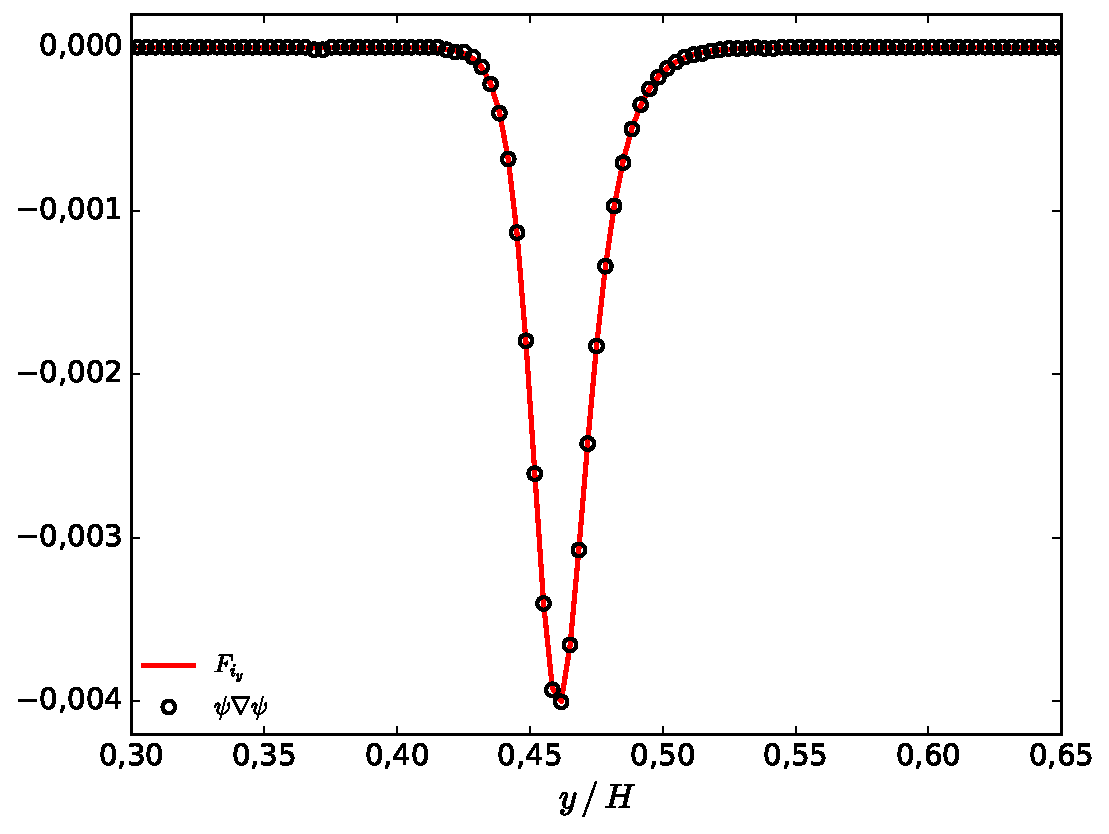
\includegraphics[width=0.75\textwidth]{vdWColumn/Fuerza/vdWcolumn_fuerza}
	\caption{Perfiles de densidad para la fuerza de interacci\'on y $\psi d\psi / dy$.}
	\label{fig:vdWColumn_TUniform_fuerza}
\end{figure}

La \eq{eq:li_macro_1d_peos} es similar al balance hidrost\'atico empleado por Berberan-Santos (\eq{eq:p_hidrost}) excepto por el t\'ermino adicional $- 2 G^2 c^4 \sigma \frac{\partial}{\partial y} \left( \left| \frac{\partial \psi}{\partial y} \right|^2  \right)$. A pesar que esta ecuaci\'on es igual a la \eq{eq:f_int_taylor} en casi todo el dominio, como se muestra en la \fig{fig:vdWColumn_fuerza_terminos}, $- 2 G^2 c^4 \sigma \frac{\partial}{\partial y} \left( \left| \frac{\partial \psi}{\partial y} \right|^2  \right)$ es diferente de cero s\'olo en las cercan\'ias de la interfase, y aunque es de un orden de magnitud menor que los principales t\'erminos de la \eq{eq:li_macro_1d}, es capaz de afectar el comportamiento de las variables macrosc\'opicas para producir el perfil de densidad continuo y difuso a trav\'es de la interfase.


\begin{figure}[ht]
	\centering
	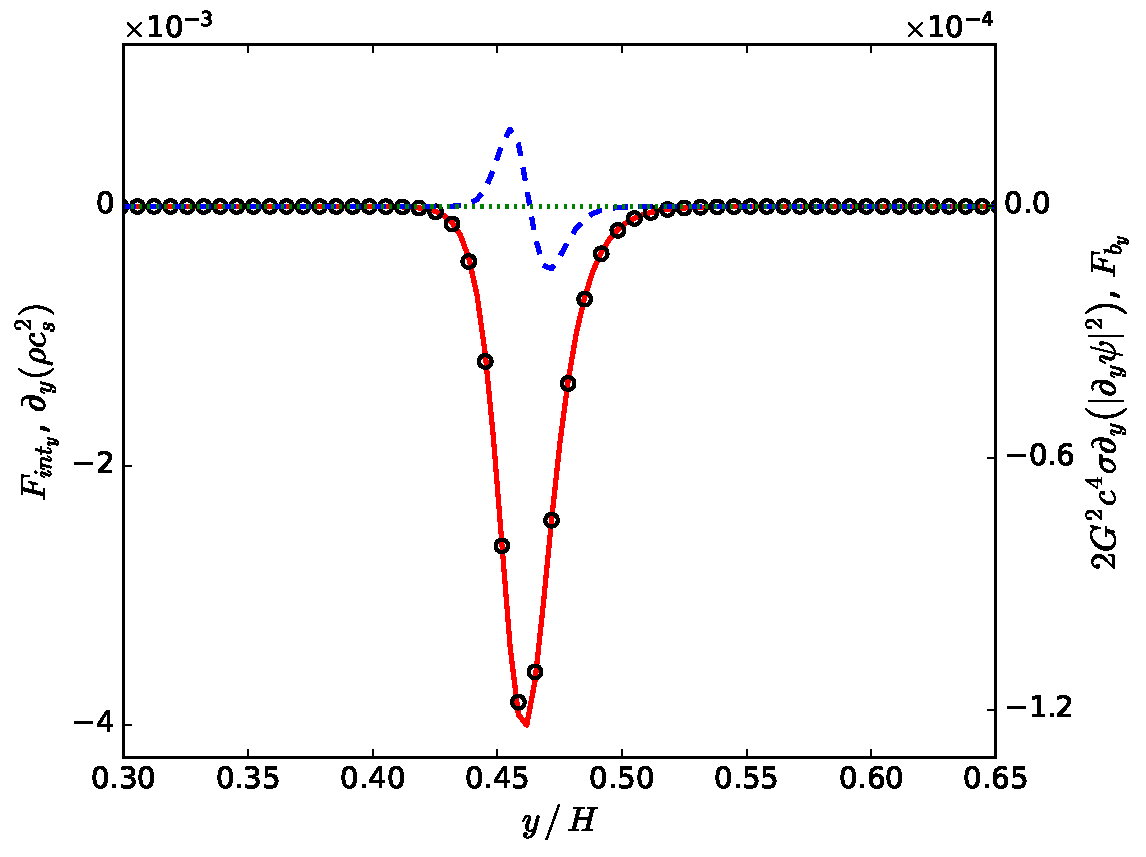
\includegraphics[width=0.75\textwidth]{vdWColumn/Fuerza_componentes/vdWcolumn_fuerza_comp}
	\caption{Distribuci\'on espacial de los diferentes componentes de la \eq{eq:li_macro_1d_peos}.}
	\label{fig:vdWColumn_fuerza_terminos}
\end{figure}
\FloatBarrier